\documentclass[11pt, letterpaper]{article}

% Fonts and Encoding
\usepackage[utf8]{inputenc}
\usepackage[T1]{fontenc}
\usepackage{lmodern} % High-quality Latin Modern vector font

% Math and Symbols
\usepackage{amsmath, amssymb, amsthm, amsfonts, mathrsfs, mathtools}

% Layout and Geometry
\usepackage{geometry}
\geometry{letterpaper, margin=1in}
\setlength{\parindent}{0pt}
\setlength{\parskip}{0.6em}

% Formatting and Graphics
\usepackage{graphicx, xcolor, enumitem, booktabs, array, tabularx}

% TikZ for Illustrations
\usepackage{tikz}
\usetikzlibrary{arrows.meta, positioning, shapes.geometric, calc, backgrounds, matrix}

% Clickable Links and TOC
\usepackage{hyperref}
\hypersetup{
    colorlinks=true,
    linkcolor=blue,
    filecolor=magenta,      
    urlcolor=cyan,
    pdftitle={Denumerable Sets},
}

% Theorem Environments
\newtheorem{theorem}{Theorem}[section]
\newtheorem{lemma}[theorem]{Lemma}
\newtheorem{proposition}[theorem]{Proposition}
\newtheorem{corollary}[theorem]{Corollary}
\theoremstyle{definition}
\newtheorem{definition}{Definition}[section]
\newtheorem{axiom}{Axiom}[section]
\newtheorem{example}{Example}[section]
\theoremstyle{remark}
\newtheorem{remark}{Remark}[section]

% Custom Commands (Enforced standard notation)
\newcommand{\R}{\mathbb{R}}
\newcommand{\N}{\mathbb{N}}
\newcommand{\Z}{\mathbb{Z}}
\newcommand{\Q}{\mathbb{Q}}
\newcommand{\E}{\mathbb{E}}
\newcommand{\Prob}{\mathbb{P}}
\newcommand{\F}{\mathcal{F}}

\title{\textbf{Denumerable Sets: Foundations of Countable Infinity, Rigorous Proofs, and Quantitative Modeling}}
\author{Tashfeen Omran}
\date{\today}

\begin{document}

\maketitle
\tableofcontents
\newpage

% ==============================================================================
% PART 1
% ==============================================================================
\section{Comprehensive Introduction, Context, and Prerequisites}

\subsection{Core Concepts and Axioms}

The study of \textbf{Denumerable Sets} marks the rigorous transition from finite combinatorics to the arithmetic and structure of infinite sets. Whereas finite sets have cardinalities measured by natural numbers $0, 1, 2, \dots, n$, infinite sets require a relational definition of size rooted entirely in functions. Throughout this document, we adhere to the standard convention in Section 11.2 that $\mathbb{N} = \{1, 2, 3, \dots\}$ denotes the set of positive integers.

\begin{definition}[Numerical Equivalence and Cardinality]
Two sets $A$ and $B$ are said to be \textbf{numerically equivalent} (or to have the \textbf{same cardinality}), denoted $|A| = |B|$, if there exists a bijective (one-to-one and onto) function $f : A \to B$.
\end{definition}

\begin{definition}[Denumerable, Countable, and Uncountable Sets]
Let $A$ be a set.
\begin{enumerate}[label=(\alph*)]
    \item $A$ is \textbf{denumerable} (or \textbf{countably infinite}) if $|A| = |\mathbb{N}|$; that is, there exists a bijection $f : \mathbb{N} \to A$.
    \item $A$ is \textbf{countable} if $A$ is either finite or denumerable.
    \item $A$ is \textbf{uncountable} if $A$ is not countable (and hence necessarily infinite).
\end{enumerate}
\end{definition}

\begin{definition}[Sequential Enumeration Criterion]
A set $A$ is denumerable if and only if its elements can be listed as an infinite sequence of distinct terms $a_1, a_2, a_3, \dots$ such that $A = \{a_1, a_2, a_3, \dots\}$ and $a_i \neq a_j$ whenever $i \neq j$. In this representation, the defining bijection $f : \mathbb{N} \to A$ is given by $f(n) = a_n$ for every $n \in \mathbb{N}$.
\end{definition}

\begin{axiom}[Well-Ordering Principle for $\mathbb{N}$]
Every nonempty subset $S \subseteq \mathbb{N}$ contains a least (smallest) element; that is, there exists $m \in S$ such that $m \leq s$ for all $s \in S$.
\end{axiom}

The Well-Ordering Principle is logically equivalent to the Principle of Mathematical Induction and plays a central structural role in proving that infinite subsets of denumerable sets remain denumerable (Theorem 11.4). Additionally, when dealing with countable collections of arbitrary denumerable sets (such as Exercise 11.16), one implicitly relies on the \textbf{Axiom of Countable Choice}, which permits simultaneously selecting one bijection $g_i : \mathbb{N} \to A_i$ for each $i \in \mathbb{N}$.

\subsection{Intuition and Set-Theoretic/Logical Foundations}

To understand denumerable sets intuitively, imagine an infinite hotel (Hilbert's Hotel) with rooms numbered $1, 2, 3, \dots$ corresponding to $\mathbb{N}$. A set $A$ is denumerable precisely when every element of $A$ can be assigned a unique room number such that no room is left vacant.

This functional perspective immediately disrupts our finite-set intuition:
\begin{itemize}
    \item \textbf{Proper Subsets of Equal Size:} For finite sets, a proper subset $B \subsetneq A$ always has strictly smaller cardinality ($|B| < |A|$). For infinite sets, this fails dramatically. For instance, $\mathbb{N} \subsetneq \mathbb{Z}$, yet $|\mathbb{N}| = |\mathbb{Z}|$ because we can interleave positive and non-positive integers: $0, 1, -1, 2, -2, \dots$. This property---having the same cardinality as a proper subset---is in fact the defining characteristic of Dedekind-infinite sets.
    \item \textbf{Ordering and Traversal:} A two-dimensional grid $\mathbb{N} \times \mathbb{N}$ appears ``larger'' than the one-dimensional line $\mathbb{N}$. However, cardinality ignores geometric dimension and density; it asks only whether a one-to-one pairing exists. If one traverses $\mathbb{N} \times \mathbb{N}$ row-by-row, one gets stuck in the infinite first row and never reaches row $2$. By instead traversing along finite anti-diagonals ($i + j = k$), every grid point is reached in finitely many steps, yielding a bijection $\mathbb{N} \to \mathbb{N} \times \mathbb{N}$.
    \item \textbf{Handling Redundancies:} When enumerating $\mathbb{Q}^+$ via the grid $j/i$, every positive rational number appears infinitely often (e.g., $1/2 = 2/4 = 3/6 = \dots$). A naive traversal gives a surjection $\mathbb{N} \to \mathbb{Q}^+$, not a bijection. By skipping previously encountered values during the diagonal traversal, we systematically purge duplicates to preserve injectivity while retaining surjectivity.
\end{itemize}

\subsection{Historical Context and Motivation}

Before the late nineteenth century, mathematicians largely treated infinity as a purely potential process (``growing without bound'') rather than a completed mathematical object. Galileo Galilei famously noted in his 1638 \textit{Discorsi} that the positive integers $\{1, 2, 3, \dots\}$ could be placed in one-to-one correspondence with their squares $\{1, 4, 9, \dots\}$, concluding somewhat uneasily that the notions of ``less than,'' ``equal to,'' and ``greater than'' do not apply to the infinite.

The formalization of denumerable sets emerged in the 1870s through the pioneering work of \textbf{Georg Cantor} on trigonometric series and real analysis. While investigating sets of points where a Fourier series could fail to converge, Cantor realized he needed to classify the ``sizes'' of infinite subsets of $\mathbb{R}$. In 1874, Cantor published his landmark paper demonstrating two revolutionary facts: first, that the set of algebraic numbers (and hence $\mathbb{Q}$) is denumerable despite being dense in $\mathbb{R}$; and second, that $\mathbb{R}$ itself is \textit{not} denumerable. This discovery shattered the monolithic view of infinity, gave birth to modern set theory, and catalyzed the foundational debates of the early twentieth century (including Zermelo-Fraenkel set theory and the Axiom of Choice), which in turn laid the axiomatic bedrock for Kolmogorov's measure-theoretic probability in 1933.

\subsection{Key Theorems, Lemmas, and Formulas}

The foundational results of Section 11.2 are summarized below:

\begin{theorem}[Denumerability of $\mathbb{Z}$ --- Result 11.3]
The set $\mathbb{Z}$ of all integers is denumerable. Specifically, the function $f : \mathbb{N} \to \mathbb{Z}$ defined by
\[
f(n) = \frac{1 + (-1)^n (2n - 1)}{4}
\]
is a bijection, generating the sequence $0, 1, -1, 2, -2, \dots$.
\end{theorem}

\begin{theorem}[Infinite Subsets of Denumerable Sets --- Theorem 11.4]
Every infinite subset of a denumerable set is denumerable. Equivalently, every subset of a countable set is countable.
\end{theorem}

\begin{corollary}[Even Integers and Multiples --- Result 11.5]
The set $2\mathbb{Z} = \{2n : n \in \mathbb{Z}\}$ of even integers is denumerable. More generally, $k\mathbb{Z}$ and $k\mathbb{N}$ are denumerable for every nonzero integer $k$.
\end{corollary}

\begin{theorem}[Cartesian Product of Denumerable Sets --- Result 11.6]
If $A$ and $B$ are denumerable sets, then the Cartesian product $A \times B = \{(a, b) : a \in A, b \in B\}$ is denumerable.
\end{theorem}

\begin{theorem}[Denumerability of $\mathbb{Q}^+$ and $\mathbb{Q}$ --- Results 11.7 and 11.8]
Both the set $\mathbb{Q}^+$ of positive rational numbers and the set $\mathbb{Q}$ of all rational numbers are denumerable.
\end{theorem}

\begin{proposition}[Symmetry and Transitivity of Numerical Equivalence]
For any sets $A, B, C$:
\begin{enumerate}[label=(\roman*)]
    \item If $f : A \to B$ is bijective, then $f^{-1} : B \to A$ is bijective, so $|A| = |B| \iff |B| = |A|$.
    \item If $f : A \to B$ and $g : B \to C$ are bijective, then $g \circ f : A \to C$ is bijective, so $|A| = |B|$ and $|B| = |C|$ imply $|A| = |C|$.
\end{enumerate}
\end{proposition}

\subsection{Prerequisites}

Mastery of Section 11.2 requires proficiency in the following foundational topics:
\begin{itemize}
    \item \textbf{Naive Set Theory:} Set builder notation, subsets ($B \subseteq A$), proper subsets ($B \subsetneq A$), set differences ($A - B$), pairwise disjointness ($A_i \cap A_j = \emptyset$ for $i \neq j$), and indexed unions ($\bigcup_{i=1}^\infty A_i$).
    \item \textbf{Functions and Relations:} Proving injectivity ($f(x_1) = f(x_2) \implies x_1 = x_2$), surjectivity ($\forall y \in B, \exists x \in A \text{ with } f(x) = y$), well-definedness, inverse functions, and function composition.
    \item \textbf{Proof Techniques:} Direct proof, proof by contradiction, proof by cases (e.g., parity arguments), mathematical induction, and applications of the Well-Ordering Principle on $\mathbb{N}$.
    \item \textbf{Elementary Number Theory:} Properties of even/odd integers, prime factorization (or extracting the largest power of $2$ dividing an integer), and the irrationality of $\sqrt{2}$.
\end{itemize}

% ==============================================================================
% PART 2
% ==============================================================================
\section{Detailed Homework Solutions (Section 11.2 Exercises)}

\subsection*{Exercise 11.3}
\textbf{Original Problem:} Prove that if $A$ and $B$ are disjoint denumerable sets, then $A \cup B$ is denumerable.

\begin{proof}[Proof (Direct Proof via Explicit Bijection)]
Since $A$ and $B$ are denumerable, by definition there exist bijective functions $g : \mathbb{N} \to A$ and $h : \mathbb{N} \to B$. Thus, we may list their elements as
\[
A = \{a_1, a_2, a_3, \dots\} \quad \text{and} \quad B = \{b_1, b_2, b_3, \dots\},
\]
where $a_k = g(k)$ and $b_k = h(k)$ for each $k \in \mathbb{N}$, with $a_i \neq a_j$ and $b_i \neq b_j$ whenever $i \neq j$. Furthermore, because $A$ and $B$ are disjoint, $A \cap B = \emptyset$, so $a_i \neq b_j$ for all $i, j \in \mathbb{N}$.

Define a function $f : \mathbb{N} \to A \cup B$ by interleaving the two lists:
\[
f(n) =
\begin{cases}
a_{(n+1)/2} & \text{if } n \text{ is odd}, \\
b_{n/2} & \text{if } n \text{ is even}.
\end{cases}
\]
We verify that $f$ is well-defined, injective, and surjective.
\begin{enumerate}[label=(\arabic*)]
    \item \textbf{Well-definedness:} If $n \in \mathbb{N}$ is odd, then $n = 2k - 1$ for some $k \in \mathbb{N}$, so $(n+1)/2 = k \in \mathbb{N}$ and $f(n) = a_k \in A \subseteq A \cup B$. If $n \in \mathbb{N}$ is even, then $n = 2k$ for some $k \in \mathbb{N}$, so $n/2 = k \in \mathbb{N}$ and $f(n) = b_k \in B \subseteq A \cup B$. Thus every $n \in \mathbb{N}$ maps to a unique element of $A \cup B$.
    
    \item \textbf{Injectivity:} Suppose $f(m) = f(n)$ for some $m, n \in \mathbb{N}$. We examine the parity of $m$ and $n$:
    \begin{itemize}
        \item \textit{Case 1 ($m$ and $n$ have opposite parity):} Without loss of generality, assume $m$ is odd and $n$ is even. Then $f(m) \in A$ and $f(n) \in B$. Since $f(m) = f(n)$, this implies $f(m) \in A \cap B$, contradicting $A \cap B = \emptyset$. Thus this case cannot occur.
        \item \textit{Case 2 ($m$ and $n$ are both odd):} Then $a_{(m+1)/2} = a_{(n+1)/2}$, i.e., $g((m+1)/2) = g((n+1)/2)$. Since $g$ is injective, $(m+1)/2 = (n+1)/2$, which yields $m = n$.
        \item \textit{Case 3 ($m$ and $n$ are both even):} Then $b_{m/2} = b_{n/2}$, i.e., $h(m/2) = h(n/2)$. Since $h$ is injective, $m/2 = n/2$, which yields $m = n$.
    \end{itemize}
    Hence $f$ is one-to-one.
    
    \item \textbf{Surjectivity:} Let $x \in A \cup B$ be arbitrary. By definition of set union, either $x \in A$ or $x \in B$.
    \begin{itemize}
        \item If $x \in A$, then since $g$ is surjective, there exists $k \in \mathbb{N}$ such that $x = g(k) = a_k$. Choosing $n = 2k - 1 \in \mathbb{N}$ (which is odd), we obtain $f(2k - 1) = a_{((2k-1)+1)/2} = a_k = x$.
        \item If $x \in B$, then since $h$ is surjective, there exists $k \in \mathbb{N}$ such that $x = h(k) = b_k$. Choosing $n = 2k \in \mathbb{N}$ (which is even), we obtain $f(2k) = b_{2k/2} = b_k = x$.
    \end{itemize}
    Hence $f$ is onto.
\end{enumerate}
Since $f : \mathbb{N} \to A \cup B$ is bijective, $|A \cup B| = |\mathbb{N}|$, and therefore $A \cup B$ is denumerable. $\blacksquare$
\end{proof}

\subsection*{Exercise 11.4}
\textbf{Original Problem:} Let $\mathbb{R}^+$ denote the set of positive real numbers and let $A$ and $B$ be denumerable subsets of $\mathbb{R}^+$. Define $C = \{x \in \mathbb{R} : -x \in B\}$. Show that $A \cup C$ is denumerable.

\begin{proof}[Proof (Direct Proof via Bijection and Reduction to Exercise 11.3)]
Our strategy is to prove that $C$ is denumerable and disjoint from $A$, and then invoke Exercise 11.3.

First, define a function $\phi : B \to C$ by $\phi(y) = -y$ for all $y \in B$.
\begin{itemize}
    \item \textit{Well-definedness:} For every $y \in B$, we have $-(-y) = y \in B$, so $-y \in C$ by definition of $C$.
    \item \textit{Injectivity:} If $\phi(y_1) = \phi(y_2)$, then $-y_1 = -y_2$, which implies $y_1 = y_2$.
    \item \textit{Surjectivity:} Let $x \in C$. By definition of $C$, $y = -x \in B$. Then $\phi(y) = -(-x) = x$.
\end{itemize}
Thus $\phi : B \to C$ is a bijection, so $|C| = |B|$. Because $B$ is denumerable, there exists a bijection $h : \mathbb{N} \to B$. The composition $\phi \circ h : \mathbb{N} \to C$ is a composition of bijections and hence is a bijection from $\mathbb{N}$ to $C$. Therefore, $C$ is denumerable.

Next, we prove that $A \cap C = \emptyset$. Suppose for contradiction that there exists $z \in A \cap C$. Since $z \in A \subseteq \mathbb{R}^+$, we must have $z > 0$. Since $z \in C$, by definition $-z \in B \subseteq \mathbb{R}^+$, which implies $-z > 0$, or equivalently $z < 0$. This yields $0 < z < 0$, a contradiction. Hence $A \cap C = \emptyset$.

Since $A$ and $C$ are disjoint denumerable sets, it follows directly from Exercise 11.3 that $A \cup C$ is denumerable. $\blacksquare$
\end{proof}

\subsection*{Exercise 11.5}
\textbf{Original Problem:} Prove that $|\mathbb{Z}| = |\mathbb{Z} - \{2\}|$.

\begin{proof}[Proof (Direct Proof via Explicit Bijection)]
Define a function $f : \mathbb{Z} \to \mathbb{Z} - \{2\}$ by
\[
f(n) =
\begin{cases}
n & \text{if } n < 2, \\
n + 1 & \text{if } n \geq 2.
\end{cases}
\]
We verify that $f$ is well-defined, injective, and surjective.
\begin{enumerate}[label=(\arabic*)]
    \item \textbf{Well-definedness:} Let $n \in \mathbb{Z}$. If $n < 2$, then $f(n) = n \in \mathbb{Z}$ and $f(n) < 2$, so $f(n) \neq 2$. If $n \geq 2$, then $f(n) = n + 1 \in \mathbb{Z}$ and $f(n) \geq 3 > 2$, so $f(n) \neq 2$. In both cases, $f(n) \in \mathbb{Z} - \{2\}$.
    
    \item \textbf{Injectivity:} Suppose $f(m) = f(n)$ for $m, n \in \mathbb{Z}$.
    \begin{itemize}
        \item If $m < 2$ and $n < 2$, then $f(m) = f(n) \implies m = n$.
        \item If $m \geq 2$ and $n \geq 2$, then $f(m) = f(n) \implies m + 1 = n + 1 \implies m = n$.
        \item If $m < 2$ and $n \geq 2$ (or symmetrically $n < 2$ and $m \geq 2$), then $f(m) = m < 2 < 3 \leq n + 1 = f(n)$, so $f(m) \neq f(n)$, a contradiction.
    \end{itemize}
    Thus $m = n$, so $f$ is one-to-one.
    
    \item \textbf{Surjectivity:} Let $y \in \mathbb{Z} - \{2\}$. Since $y \in \mathbb{Z}$ and $y \neq 2$, either $y < 2$ or $y > 2$.
    \begin{itemize}
        \item If $y < 2$, choose $n = y \in \mathbb{Z}$. Since $n < 2$, $f(n) = n = y$.
        \item If $y > 2$, then since $y$ is an integer, $y \geq 3$. Choose $n = y - 1 \in \mathbb{Z}$. Then $n \geq 2$, so $f(n) = (y - 1) + 1 = y$.
    \end{itemize}
    Thus $f$ is onto.
\end{enumerate}
Since $f : \mathbb{Z} \to \mathbb{Z} - \{2\}$ is bijective, we conclude by definition of numerical equivalence that $|\mathbb{Z}| = |\mathbb{Z} - \{2\}|$. $\blacksquare$
\end{proof}

\subsection*{Exercise 11.6}
\textbf{Original Problem:}
\begin{enumerate}[label=(\alph*)]
    \item Prove that the function $f : \mathbb{R} - \{1\} \to \mathbb{R} - \{2\}$ defined by $f(x) = \frac{2x}{x-1}$ is bijective.
    \item Explain why $|\mathbb{R} - \{1\}| = |\mathbb{R} - \{2\}|$.
\end{enumerate}

\begin{proof}[Proof (Direct Verification of Bijection)]
\textbf{Part (a):} We establish well-definedness, injectivity, and surjectivity for $f$.
\begin{enumerate}[label=(\arabic*)]
    \item \textbf{Well-definedness:} Let $x \in \mathbb{R} - \{1\}$. Because $x \neq 1$, the denominator $x - 1 \neq 0$, so $\frac{2x}{x-1} \in \mathbb{R}$ is well-defined. Moreover, we must check that $f(x) \neq 2$: if $\frac{2x}{x-1} = 2$, multiplying by $x - 1$ gives $2x = 2x - 2$, which implies $0 = -2$, a contradiction. Thus $f(x) \in \mathbb{R} - \{2\}$ for all $x \in \mathbb{R} - \{1\}$.
    
    \item \textbf{Injectivity:} Suppose $f(a) = f(b)$ for $a, b \in \mathbb{R} - \{1\}$. Then
    \[
    \frac{2a}{a - 1} = \frac{2b}{b - 1}.
    \]
    Since $a - 1 \neq 0$ and $b - 1 \neq 0$, cross-multiplying gives
    \[
    2a(b - 1) = 2b(a - 1) \implies 2ab - 2a = 2ab - 2b \implies -2a = -2b \implies a = b.
    \]
    Hence $f$ is one-to-one.
    
    \item \textbf{Surjectivity:} Let $y \in \mathbb{R} - \{2\}$. Define $x = \frac{y}{y - 2}$. Since $y \neq 2$, the denominator $y - 2 \neq 0$, so $x \in \mathbb{R}$. Furthermore, $x \neq 1$, because if $\frac{y}{y - 2} = 1$, then $y = y - 2$, yielding $0 = -2$, a contradiction. Therefore $x \in \mathbb{R} - \{1\}$. Evaluating $f(x)$ gives
    \[
    f(x) = f\left(\frac{y}{y - 2}\right) = \frac{2\left(\frac{y}{y - 2}\right)}{\frac{y}{y - 2} - 1} = \frac{\frac{2y}{y - 2}}{\frac{y - (y - 2)}{y - 2}} = \frac{2y}{2} = y.
    \]
    Hence $f$ is onto.
\end{enumerate}
Therefore, $f : \mathbb{R} - \{1\} \to \mathbb{R} - \{2\}$ is bijective.

\textbf{Part (b):} By the definition of cardinality (numerical equivalence), two sets $A$ and $B$ satisfy $|A| = |B|$ if and only if there exists a bijective function from $A$ to $B$. Since part (a) established that $f : \mathbb{R} - \{1\} \to \mathbb{R} - \{2\}$ is bijective, it follows immediately that $|\mathbb{R} - \{1\}| = |\mathbb{R} - \{2\}|$. $\blacksquare$
\end{proof}

\subsection*{Exercise 11.7}
\textbf{Original Problem:} Let
\[
S = \left\{ x \in \mathbb{R} : x = \frac{n^2 + \sqrt{2}}{n},\ n \in \mathbb{N} \right\}.
\]
Define $f : \mathbb{N} \to S$ by $f(n) = \frac{n^2 + \sqrt{2}}{n}$.
\begin{enumerate}[label=(\alph*)]
    \item List three elements that belong to $S$.
    \item Show that $f$ is one-to-one.
    \item Show that $f$ is onto.
    \item Is $S$ denumerable? Explain.
\end{enumerate}

\begin{proof}[Solution and Proof (Direct Verification and Contradiction)]
\textbf{Part (a):} Evaluating $f(n)$ for $n = 1, 2, 3 \in \mathbb{N}$ yields three elements of $S$:
\[
f(1) = \frac{1^2 + \sqrt{2}}{1} = 1 + \sqrt{2}, \qquad f(2) = \frac{2^2 + \sqrt{2}}{2} = 2 + \frac{\sqrt{2}}{2}, \qquad f(3) = \frac{3^2 + \sqrt{2}}{3} = 3 + \frac{\sqrt{2}}{3}.
\]

\textbf{Part (b):} We prove $f$ is one-to-one by contradiction. Suppose $f(m) = f(n)$ for some $m, n \in \mathbb{N}$, and assume toward a contradiction that $m \neq n$. Then
\[
\frac{m^2 + \sqrt{2}}{m} = \frac{n^2 + \sqrt{2}}{n} \implies m + \frac{\sqrt{2}}{m} = n + \frac{\sqrt{2}}{n}.
\]
Rearranging terms gives
\[
m - n = \sqrt{2}\left(\frac{1}{n} - \frac{1}{m}\right) = \sqrt{2}\left(\frac{m - n}{mn}\right).
\]
Since $m \neq n$, we have $m - n \neq 0$, so we may divide both sides by $m - n$ to obtain
\[
1 = \frac{\sqrt{2}}{mn} \implies \sqrt{2} = mn.
\]
Because $m, n \in \mathbb{N}$, their product $mn$ is a positive integer ($mn \in \mathbb{N} \subseteq \mathbb{Q}$). However, $\sqrt{2}$ is irrational ($\sqrt{2} \notin \mathbb{Q}$), which is a contradiction. Therefore $m = n$, proving that $f$ is one-to-one.

\textbf{Part (c):} Let $x \in S$ be arbitrary. By the set-builder definition of $S$, there exists $n \in \mathbb{N}$ such that $x = \frac{n^2 + \sqrt{2}}{n}$. By the definition of $f$, we have $f(n) = \frac{n^2 + \sqrt{2}}{n} = x$. Hence $f$ is onto.

\textbf{Part (d):} Yes, $S$ is denumerable. By parts (b) and (c), the function $f : \mathbb{N} \to S$ is both one-to-one and onto, so $f$ is bijective. By definition, $|S| = |\mathbb{N}|$, which means $S$ is denumerable. $\blacksquare$
\end{proof}

\subsection*{Exercise 11.8}
\textbf{Original Problem:} Prove that the function $f : \mathbb{N} \to \mathbb{Z}$ defined in (11.1) by $f(n) = \frac{1 + (-1)^n(2n - 1)}{4}$ is bijective.

\begin{proof}[Proof (Direct Proof by Parity Cases)]
First, we verify that $f$ is well-defined (i.e., $f(n) \in \mathbb{Z}$ for all $n \in \mathbb{N}$) and express $f$ piecewise according to the parity of $n$:
\begin{itemize}
    \item If $n \in \mathbb{N}$ is even, write $n = 2k$ for a unique $k \in \mathbb{N}$. Then $(-1)^{2k} = 1$, so
    \[
    f(2k) = \frac{1 + 1\cdot(4k - 1)}{4} = \frac{4k}{4} = k \in \mathbb{Z}^+.
    \]
    \item If $n \in \mathbb{N}$ is odd, write $n = 2k - 1$ for a unique $k \in \mathbb{N}$. Then $(-1)^{2k-1} = -1$, so
    \[
    f(2k - 1) = \frac{1 - (2(2k - 1) - 1)}{4} = \frac{1 - (4k - 3)}{4} = \frac{4 - 4k}{4} = 1 - k \in \mathbb{Z}_{\leq 0}.
    \]
\end{itemize}
Since every $n \in \mathbb{N}$ is either even or odd, $f(n) \in \mathbb{Z}$ for all $n \in \mathbb{N}$, so $f$ is well-defined.

\textbf{Injectivity:} Suppose $f(m) = f(n)$ for $m, n \in \mathbb{N}$. Observe from the formulas above that if $r$ is even, $f(r) = r/2 \geq 1 > 0$, whereas if $r$ is odd, $f(r) = 1 - (r+1)/2 = (1 - r)/2 \leq 0$. Because positive integers and non-positive integers are disjoint, $m$ and $n$ must have the same parity:
\begin{itemize}
    \item \textit{Case 1 ($m = 2j$ and $n = 2k$ are both even, $j, k \in \mathbb{N}$):} Then $f(m) = f(n)$ yields $j = k$, so $m = 2j = 2k = n$.
    \item \textit{Case 2 ($m = 2j - 1$ and $n = 2k - 1$ are both odd, $j, k \in \mathbb{N}$):} Then $f(m) = f(n)$ yields $1 - j = 1 - k$, so $j = k$, and hence $m = 2j - 1 = 2k - 1 = n$.
\end{itemize}
Therefore, $f$ is one-to-one.

\textbf{Surjectivity:} Let $z \in \mathbb{Z}$ be arbitrary. We consider two exhaustive cases:
\begin{itemize}
    \item \textit{Case 1 ($z \geq 1$):} Let $n = 2z$. Since $z \in \mathbb{N}$, $n = 2z \in \mathbb{N}$ is even, and $f(n) = f(2z) = z$.
    \item \textit{Case 2 ($z \leq 0$):} Let $k = 1 - z$. Since $z \leq 0$, we have $k \geq 1$, so $k \in \mathbb{N}$. Setting $n = 2k - 1 = 1 - 2z \in \mathbb{N}$ (which is odd), we obtain $f(n) = f(2k - 1) = 1 - k = 1 - (1 - z) = z$.
\end{itemize}
Thus every $z \in \mathbb{Z}$ has a preimage in $\mathbb{N}$, so $f$ is onto.

Since $f$ is both one-to-one and onto, $f : \mathbb{N} \to \mathbb{Z}$ is bijective. $\blacksquare$
\end{proof}

\subsection*{Exercise 11.9}
\textbf{Original Problem:} Show that every denumerable set $A$ can be partitioned into two denumerable subsets of $A$.

\begin{proof}[Proof (Constructive Proof via Parity Partition of Indices)]
Let $A$ be a denumerable set. By definition, there exists a bijection $f : \mathbb{N} \to A$, allowing us to write $A = \{a_1, a_2, a_3, \dots\}$ where $a_n = f(n)$ for each $n \in \mathbb{N}$ and $a_i \neq a_j$ whenever $i \neq j$.

Define two subsets of $A$ corresponding to odd and even indices:
\[
A_1 = \{a_{2k - 1} : k \in \mathbb{N}\} = \{a_1, a_3, a_5, \dots\} \quad \text{and} \quad A_2 = \{a_{2k} : k \in \mathbb{N}\} = \{a_2, a_4, a_6, \dots\}.
\]
We verify two claims: (i) $\{A_1, A_2\}$ is a partition of $A$, and (ii) both $A_1$ and $A_2$ are denumerable.

\begin{enumerate}[label=(\arabic*)]
    \item \textbf{Partition Verification:}
    \begin{itemize}
        \item \textit{Nonemptiness:} $a_1 = a_{2(1)-1} \in A_1$ and $a_2 = a_{2(1)} \in A_2$, so $A_1 \neq \emptyset$ and $A_2 \neq \emptyset$.
        \item \textit{Disjointness:} Suppose $x \in A_1 \cap A_2$. Then $x = a_{2j - 1} = a_{2k}$ for some $j, k \in \mathbb{N}$, i.e., $f(2j - 1) = f(2k)$. Since $f$ is injective, $2j - 1 = 2k$. This is impossible because $2j - 1$ is odd while $2k$ is even. Thus $A_1 \cap A_2 = \emptyset$.
        \item \textit{Exhaustiveness:} Clearly $A_1 \cup A_2 \subseteq A$ since each $A_i \subseteq A$. Conversely, let $a \in A$. Because $f$ is surjective, $a = a_n$ for some $n \in \mathbb{N}$. If $n$ is odd, then $n = 2k - 1$ for $k = (n+1)/2 \in \mathbb{N}$, so $a \in A_1$. If $n$ is even, then $n = 2k$ for $k = n/2 \in \mathbb{N}$, so $a \in A_2$. Hence $A \subseteq A_1 \cup A_2$, proving $A_1 \cup A_2 = A$.
    \end{itemize}
    
    \item \textbf{Denumerability of $A_1$ and $A_2$:} Define $g_1 : \mathbb{N} \to A_1$ by $g_1(k) = a_{2k - 1}$ and $g_2 : \mathbb{N} \to A_2$ by $g_2(k) = a_{2k}$.
    \begin{itemize}
        \item Both $g_1$ and $g_2$ are surjective onto $A_1$ and $A_2$, respectively, by the definitions of $A_1$ and $A_2$.
        \item For injectivity of $g_1$: if $g_1(j) = g_1(k)$, then $f(2j - 1) = f(2k - 1)$. Injectivity of $f$ implies $2j - 1 = 2k - 1$, so $j = k$. Similarly, $g_2(j) = g_2(k) \implies f(2j) = f(2k) \implies 2j = 2k \implies j = k$.
    \end{itemize}
    Thus $g_1$ and $g_2$ are bijections, showing $|A_1| = |A_2| = |\mathbb{N}|$.
\end{enumerate}
Therefore, $\{A_1, A_2\}$ is a partition of $A$ into two denumerable subsets. $\blacksquare$
\end{proof}

\subsection*{Exercise 11.10}
\textbf{Original Problem:} Let $A$ be a denumerable set and let $B = \{x, y\}$. Prove that $A \times B$ is denumerable.

\begin{proof}[Proof (Direct Proof by Cases and Explicit Bijection)]
Since $A$ is denumerable, there exists a bijection $g : \mathbb{N} \to A$, so we can write $A = \{a_1, a_2, a_3, \dots\}$ where $a_n = g(n)$ and $a_i \neq a_j$ for $i \neq j$. We consider whether $x$ and $y$ are distinct (noting that standard set notation $\{x, y\}$ typically implies $x \neq y$, though we address $x = y$ for complete generality):

\textit{Case 1 ($x \neq y$):} Define $f : \mathbb{N} \to A \times B$ by
\[
f(n) =
\begin{cases}
(a_{(n+1)/2},\, x) & \text{if } n \text{ is odd}, \\
(a_{n/2},\, y) & \text{if } n \text{ is even}.
\end{cases}
\]
(Alternatively, $A \times B = (A \times \{x\}) \cup (A \times \{y\})$ is a disjoint union of two denumerable sets, to which Exercise 11.3 applies.) Checking $f$ directly:
\begin{itemize}
    \item \textit{Injectivity:} Suppose $f(m) = f(n)$. Because $x \neq y$, the second coordinates of $f(m)$ and $f(n)$ can only be equal if $m$ and $n$ have the same parity. If both are odd, $(a_{(m+1)/2}, x) = (a_{(n+1)/2}, x)$ gives $a_{(m+1)/2} = a_{(n+1)/2}$, and injectivity of $g$ yields $(m+1)/2 = (n+1)/2$, so $m = n$. If both are even, $(a_{m/2}, y) = (a_{n/2}, y)$ similarly yields $m/2 = n/2$, so $m = n$.
    \item \textit{Surjectivity:} Let $(a, b) \in A \times B$. Since $g$ is surjective, $a = a_k$ for some $k \in \mathbb{N}$. Since $b \in \{x, y\}$, either $b = x$, in which case $f(2k - 1) = (a_k, x) = (a, b)$, or $b = y$, in which case $f(2k) = (a_k, y) = (a, b)$.
\end{itemize}
Thus $f$ is bijective, so $A \times B$ is denumerable.

\textit{Case 2 ($x = y$):} Then $B = \{x\}$, and $h : \mathbb{N} \to A \times \{x\}$ defined by $h(n) = (a_n, x)$ is immediately bijective (since $a_m = a_n \iff m = n$, and every $(a, x) \in A \times \{x\}$ equals $(a_n, x)$ for some $n \in \mathbb{N}$).

In either case, $A \times B$ is denumerable. $\blacksquare$
\end{proof}

\subsection*{Exercise 11.11}
\textbf{Original Problem:} Let $B$ be a denumerable set and let $A$ be a nonempty set of unspecified cardinality. If $f : A \to B$ is a one-to-one function, then what can be said about the cardinality of $A$? Explain.

\begin{proof}[Solution and Proof (Image Restriction and Theorem 11.4)]
\textbf{Conclusion:} The set $A$ must be \textbf{countable} (and nonempty); that is, $A$ is either finite (with $|A| \in \mathbb{N}$) or denumerable ($|A| = |\mathbb{N}|$).

\textbf{Explanation and Proof:} Consider the image (range) of $f$, defined by
\[
f(A) = \{f(a) : a \in A\} \subseteq B.
\]
Define a new function $\tilde{f} : A \to f(A)$ by $\tilde{f}(a) = f(a)$ for every $a \in A$ (restricting the codomain of $f$ to its range).
\begin{itemize}
    \item Because $f$ is one-to-one, if $\tilde{f}(a_1) = \tilde{f}(a_2)$, then $f(a_1) = f(a_2)$, so $a_1 = a_2$. Hence $\tilde{f}$ is one-to-one.
    \item By definition of $f(A)$, every element $b \in f(A)$ satisfies $b = f(a) = \tilde{f}(a)$ for at least one $a \in A$. Hence $\tilde{f}$ is onto $f(A)$.
\end{itemize}
Therefore, $\tilde{f} : A \to f(A)$ is bijective, which implies $|A| = |f(A)|$.

Now $f(A)$ is a nonempty subset of the denumerable set $B$ (nonempty because $A \neq \emptyset$). There are two mutually exclusive possibilities for $f(A)$:
\begin{enumerate}[label=(\arabic*)]
    \item If $f(A)$ is finite, then since $|A| = |f(A)|$, $A$ is finite (specifically, $|A| = n$ for some $n \in \mathbb{N}$), and hence $A$ is countable. (For example, $A = \{1, 2, \dots, n\}$ and $B = \mathbb{N}$ with $f(x) = x$ achieves any finite size $n \geq 1$.)
    \item If $f(A)$ is infinite, then since $f(A) \subseteq B$ and $B$ is denumerable, Theorem 11.4 guarantees that $f(A)$ is denumerable. Because $|A| = |f(A)|$ and $|f(A)| = |\mathbb{N}|$, transitivity of numerical equivalence implies $|A| = |\mathbb{N}|$, so $A$ is denumerable, and hence countable. (For example, $A = B = \mathbb{N}$ with $f(x) = x$ achieves this.)
\end{enumerate}
Thus, in all cases, $A$ is a nonempty countable set (finite or denumerable), and it cannot be uncountable. $\blacksquare$
\end{proof}

\subsection*{Exercise 11.12}
\textbf{Original Problem:} Prove that the set of all $2$-element subsets of $\mathbb{N}$ is denumerable.

\begin{proof}[Proof (Bijection with an Infinite Subset of $\mathbb{N} \times \mathbb{N}$, Result 11.6, and Theorem 11.4)]
Let $\mathcal{P}_2(\mathbb{N}) = \{\{i, j\} : i, j \in \mathbb{N},\ i \neq j\}$ denote the set of all $2$-element subsets of $\mathbb{N}$. Define the subset $S \subseteq \mathbb{N} \times \mathbb{N}$ by
\[
S = \{(i, j) \in \mathbb{N} \times \mathbb{N} : i < j\}.
\]
First, we show that $|S| = |\mathcal{P}_2(\mathbb{N})|$ by defining $g : S \to \mathcal{P}_2(\mathbb{N})$ via $g(i, j) = \{i, j\}$.
\begin{itemize}
    \item \textit{Well-definedness:} If $(i, j) \in S$, then $i, j \in \mathbb{N}$ and $i < j$ (so $i \neq j$), meaning $\{i, j\} \in \mathcal{P}_2(\mathbb{N})$.
    \item \textit{Injectivity:} Suppose $g(i_1, j_1) = g(i_2, j_2)$ for $(i_1, j_1), (i_2, j_2) \in S$. Then $\{i_1, j_1\} = \{i_2, j_2\}$. Since $i_1 < j_1$ and $i_2 < j_2$, taking the minimum and maximum of these equal two-element sets yields
    \[
    i_1 = \min\{i_1, j_1\} = \min\{i_2, j_2\} = i_2 \quad \text{and} \quad j_1 = \max\{i_1, j_1\} = \max\{i_2, j_2\} = j_2.
    \]
    Hence $(i_1, j_1) = (i_2, j_2)$.
    \item \textit{Surjectivity:} Let $X \in \mathcal{P}_2(\mathbb{N})$. Then $X = \{a, b\}$ for two distinct natural numbers $a, b \in \mathbb{N}$. By trichotomy of order on $\mathbb{N}$, either $a < b$ or $b < a$. If $a < b$, then $(a, b) \in S$ and $g(a, b) = \{a, b\} = X$. If $b < a$, then $(b, a) \in S$ and $g(b, a) = \{b, a\} = \{a, b\} = X$.
\end{itemize}
Thus $g$ is a bijection, so $|\mathcal{P}_2(\mathbb{N})| = |S|$.

Second, we show that $S$ is denumerable. By Result 11.6, since $\mathbb{N}$ is denumerable, the Cartesian product $\mathbb{N} \times \mathbb{N}$ is denumerable. Because $S \subseteq \mathbb{N} \times \mathbb{N}$, by Theorem 11.4 it suffices to show that $S$ is infinite. Observe that for every $n \in \mathbb{N}$ with $n \geq 2$, we have $1 < n$, so $(1, n) \in S$. If $S$ were finite, say $|S| = k$ for some $k \in \mathbb{N}$, then the subset $\{(1, 2), (1, 3), \dots, (1, k + 2)\} \subseteq S$ would contain $k + 1$ distinct elements, contradicting $|S| = k$. Thus $S$ is infinite.

By Theorem 11.4, $S$ is denumerable, so $|S| = |\mathbb{N}|$. By transitivity of numerical equivalence, $|\mathcal{P}_2(\mathbb{N})| = |S| = |\mathbb{N}|$, and therefore $\mathcal{P}_2(\mathbb{N})$ is denumerable. $\blacksquare$
\end{proof}

\subsection*{Exercise 11.13}
\textbf{Original Problem:} A \textbf{Gaussian integer} is a complex number of the form $a + bi$, where $a, b \in \mathbb{Z}$ and $i = \sqrt{-1}$. Show that the set $\mathcal{G}$ of Gaussian integers is denumerable.

\begin{proof}[Proof (Bijection with $\mathbb{Z} \times \mathbb{Z}$, Result 11.3, and Result 11.6)]
By Result 11.3, the set $\mathbb{Z}$ of integers is denumerable. By Result 11.6, the Cartesian product of two denumerable sets is denumerable, so $\mathbb{Z} \times \mathbb{Z}$ is denumerable; that is, there exists a bijection $h : \mathbb{N} \to \mathbb{Z} \times \mathbb{Z}$.

Define $f : \mathbb{Z} \times \mathbb{Z} \to \mathcal{G}$ by $f(a, b) = a + bi$ for all $(a, b) \in \mathbb{Z} \times \mathbb{Z}$.
\begin{enumerate}[label=(\arabic*)]
    \item \textbf{Well-definedness and Surjectivity:} By the definition of $\mathcal{G}$, a complex number $z$ belongs to $\mathcal{G}$ if and only if there exist $a, b \in \mathbb{Z}$ such that $z = a + bi = f(a, b)$. Thus $f$ maps into $\mathcal{G}$ and is onto $\mathcal{G}$.
    
    \item \textbf{Injectivity:} Suppose $f(a_1, b_1) = f(a_2, b_2)$ for $(a_1, b_1), (a_2, b_2) \in \mathbb{Z} \times \mathbb{Z}$. Then
    \[
    a_1 + b_1 i = a_2 + b_2 i \implies a_1 - a_2 = (b_2 - b_1)i.
    \]
    If $b_1 \neq b_2$, then $b_2 - b_1 \neq 0$, allowing us to divide to obtain $i = \frac{a_1 - a_2}{b_2 - b_1} \in \mathbb{Q} \subseteq \mathbb{R}$. Squaring both sides would yield $-1 = i^2 \geq 0$ (since the square of any real number is non-negative), a contradiction. Therefore $b_1 = b_2$, which forces $a_1 - a_2 = 0$, or $a_1 = a_2$. Hence $(a_1, b_1) = (a_2, b_2)$, proving $f$ is one-to-one.
\end{enumerate}
Since $f : \mathbb{Z} \times \mathbb{Z} \to \mathcal{G}$ is bijective and $h : \mathbb{N} \to \mathbb{Z} \times \mathbb{Z}$ is bijective, their composition $f \circ h : \mathbb{N} \to \mathcal{G}$ is a bijection. Therefore, $\mathcal{G}$ is denumerable. $\blacksquare$
\end{proof}

\subsection*{Exercise 11.14}
\textbf{Original Problem:} Prove that $S = \{(a, b) : a, b \in \mathbb{N} \text{ and } b \geq 2a\}$ is denumerable.

\begin{proof}[Proof (Infinite Subset of $\mathbb{N} \times \mathbb{N}$ via Result 11.6 and Theorem 11.4)]
By definition, $S$ is a subset of $\mathbb{N} \times \mathbb{N}$. By Result 11.6, since $\mathbb{N}$ is denumerable, the Cartesian product $\mathbb{N} \times \mathbb{N}$ is denumerable. By Theorem 11.4, to conclude that $S$ is denumerable, it suffices to prove that $S$ is infinite.

For every $k \in \mathbb{N}$, consider the ordered pair $(1, 2k) \in \mathbb{N} \times \mathbb{N}$. Because $k \geq 1$, we have $2k \geq 2 = 2(1)$, which satisfies the defining condition $b \geq 2a$ of $S$. Hence $(1, 2k) \in S$ for every $k \in \mathbb{N}$. Suppose toward a contradiction that $S$ is finite, with $|S| = m$ for some non-negative integer $m$. Then the subset $\{(1, 2), (1, 4), \dots, (1, 2(m+1))\} \subseteq S$ consists of $m + 1$ distinct ordered pairs (since $2j \neq 2k$ for $j \neq k$), contradicting $|S| = m$.

Therefore, $S$ is an infinite subset of the denumerable set $\mathbb{N} \times \mathbb{N}$. By Theorem 11.4, $S$ is denumerable. $\blacksquare$
\end{proof}

\begin{remark}
Alternatively, one can construct an explicit bijection $\phi : S \to \mathbb{N} \times \mathbb{N}$ via $\phi(a, b) = (a, b - 2a + 1)$, whose inverse is $\phi^{-1}(u, v) = (u, 2u + v - 1)$.
\end{remark}

\subsection*{Exercise 11.15}
\textbf{Original Problem:} Let $S \subseteq \mathbb{N} \times \mathbb{N}$ be defined by $S = \{(i, j) : i \leq j\}$. Show that $S$ is denumerable.

\begin{proof}[Proof (Infinite Subset of $\mathbb{N} \times \mathbb{N}$ via Result 11.6 and Theorem 11.4)]
By Result 11.6, $\mathbb{N} \times \mathbb{N}$ is denumerable, and by hypothesis $S \subseteq \mathbb{N} \times \mathbb{N}$. To invoke Theorem 11.4, we verify that $S$ is infinite.

For every $n \in \mathbb{N}$, we have $1 \leq n$, so $(1, n) \in S$. If $S$ were finite with cardinality $|S| = m$ ($m \in \mathbb{Z}_{\geq 0}$), then the set $\{(1, 1), (1, 2), \dots, (1, m + 1)\} \subseteq S$ would contain $m + 1$ distinct elements, a contradiction. Hence $S$ is infinite.

Since $S$ is an infinite subset of the denumerable set $\mathbb{N} \times \mathbb{N}$, it follows from Theorem 11.4 that $S$ is denumerable. $\blacksquare$
\end{proof}

\subsection*{Exercise 11.16}
\textbf{Original Problem:} Let $A_1, A_2, A_3, \dots$ be pairwise disjoint denumerable sets. Prove that $\bigcup_{i=1}^\infty A_i$ is denumerable.

\begin{proof}[Proof (Bijection with $\mathbb{N} \times \mathbb{N}$ and Result 11.6)]
For each $i \in \mathbb{N}$, because $A_i$ is denumerable, there exists a bijection $g_i : \mathbb{N} \to A_i$. (Selecting one bijection $g_i$ for each $i \in \mathbb{N}$ uses the Axiom of Countable Choice.) Thus we can enumerate each set as
\[
A_i = \{a_{i,1}, a_{i,2}, a_{i,3}, \dots\}, \quad \text{where } a_{i,j} = g_i(j) \text{ for all } j \in \mathbb{N}.
\]
Let $U = \bigcup_{i=1}^\infty A_i$, and define a function $F : \mathbb{N} \times \mathbb{N} \to U$ by
\[
F(i, j) = a_{i,j} = g_i(j) \quad \text{for all } (i, j) \in \mathbb{N} \times \mathbb{N}.
\]
We verify that $F$ is a bijection:
\begin{enumerate}[label=(\arabic*)]
    \item \textbf{Well-definedness:} For any $(i, j) \in \mathbb{N} \times \mathbb{N}$, we have $F(i, j) = g_i(j) \in A_i \subseteq U$.
    
    \item \textbf{Injectivity:} Suppose $F(i_1, j_1) = F(i_2, j_2)$ for $(i_1, j_1), (i_2, j_2) \in \mathbb{N} \times \mathbb{N}$. Let $x = a_{i_1, j_1} = a_{i_2, j_2}$. Then $x \in A_{i_1}$ and $x \in A_{i_2}$, so $x \in A_{i_1} \cap A_{i_2}$, meaning $A_{i_1} \cap A_{i_2} \neq \emptyset$. Because the family $\{A_i\}_{i \in \mathbb{N}}$ is pairwise disjoint ($A_r \cap A_s = \emptyset$ whenever $r \neq s$), it follows that $i_1 = i_2$. Consequently, $g_{i_1}(j_1) = g_{i_1}(j_2)$. Since $g_{i_1}$ is injective, we deduce $j_1 = j_2$. Therefore $(i_1, j_1) = (i_2, j_2)$, so $F$ is one-to-one.
    
    \item \textbf{Surjectivity:} Let $x \in U = \bigcup_{i=1}^\infty A_i$. By the definition of indexed union, there exists at least one $i \in \mathbb{N}$ such that $x \in A_i$. Since $g_i : \mathbb{N} \to A_i$ is surjective, there exists $j \in \mathbb{N}$ such that $g_i(j) = x$. Thus $F(i, j) = a_{i,j} = x$, proving $F$ is onto.
\end{enumerate}
Hence $F : \mathbb{N} \times \mathbb{N} \to U$ is bijective. By Result 11.6, $\mathbb{N} \times \mathbb{N}$ is denumerable, so there exists a bijection $h : \mathbb{N} \to \mathbb{N} \times \mathbb{N}$. The composition $F \circ h : \mathbb{N} \to \bigcup_{i=1}^\infty A_i$ is a bijection, and therefore $\bigcup_{i=1}^\infty A_i$ is denumerable. $\blacksquare$
\end{proof}

\subsection*{Exercise 11.17}
\textbf{Original Problem:} Let $A = \{a_1, a_2, a_3, \dots\}$. Define $B = A - \{a_{n^2} : n \in \mathbb{N}\}$. Prove that $|A| = |B|$.

\begin{proof}[Proof (Subsets of Denumerable Sets via Theorem 11.4)]
Following the notation of Section 11.2, writing $A = \{a_1, a_2, a_3, \dots\}$ indicates that $A$ is a denumerable set whose elements $a_k$ are pairwise distinct ($a_i \neq a_j$ whenever $i \neq j$), so $|A| = |\mathbb{N}|$. By definition of set difference, $B \subseteq A$. By Theorem 11.4, if we prove that $B$ is infinite, then $B$ is denumerable, which gives $|B| = |\mathbb{N}| = |A|$.

To show $B$ is infinite, consider indices of the form $k^2 + 1$ for $k \in \mathbb{N}$. We claim that $k^2 + 1$ is never a perfect square for any $k \in \mathbb{N}$; that is, $k^2 + 1 \neq n^2$ for all $n \in \mathbb{N}$. Suppose for contradiction that $n^2 = k^2 + 1$ for some $k, n \in \mathbb{N}$. Then
\[
1 = n^2 - k^2 = (n - k)(n + k).
\]
Since $k, n \in \mathbb{N}$, we have $n + k \geq 1 + 1 = 2$, and $n - k \in \mathbb{Z}$. If $n - k \leq 0$, then $(n - k)(n + k) \leq 0 < 1$; if $n - k \geq 1$, then $(n - k)(n + k) \geq 1 \cdot 2 = 2 > 1$. In neither case can $(n - k)(n + k) = 1$, a contradiction.

Because $k^2 + 1 \neq n^2$ for all $k, n \in \mathbb{N}$ and all terms $a_i$ are distinct, $a_{k^2 + 1} \notin \{a_{n^2} : n \in \mathbb{N}\}$, so $a_{k^2 + 1} \in B$ for every $k \in \mathbb{N}$. Moreover, the map $k \mapsto a_{k^2 + 1}$ from $\mathbb{N}$ into $B$ is injective because $k_1^2 + 1 = k_2^2 + 1$ with $k_1, k_2 \in \mathbb{N}$ implies $k_1 = k_2$, and distinct indices give distinct elements of $A$. Consequently, $B$ cannot be finite (if $|B| = m$, then $\{a_{1^2+1}, a_{2^2+1}, \dots, a_{(m+1)^2+1}\} \subseteq B$ would have $m + 1$ distinct elements, contradiction).

Thus $B$ is an infinite subset of the denumerable set $A$. By Theorem 11.4, $B$ is denumerable, so $|B| = |\mathbb{N}| = |A|$. $\blacksquare$
\end{proof}

\subsection*{Exercise 11.18}
\textbf{Original Problem:} A function $f : \mathbb{N} \times \mathbb{N} \to \mathbb{N}$ is defined by $f(m, n) = 2^{m - 1}(2n - 1)$.
\begin{enumerate}[label=(\alph*)]
    \item Prove that $f$ is one-to-one and onto.
    \item Show that $\mathbb{N} \times \mathbb{N}$ is denumerable.
\end{enumerate}

\begin{proof}[Proof (Number-Theoretic Parity Argument and Well-Ordering)]
\textbf{Part (a):} First note that $f$ is well-defined: for any $m, n \in \mathbb{N}$, $m - 1 \geq 0$ implies $2^{m-1} \in \mathbb{N}$, and $n \geq 1$ implies $2n - 1 \geq 1$ is a positive integer, so $2^{m-1}(2n - 1) \in \mathbb{N}$.

\begin{enumerate}[label=(\arabic*)]
    \item \textbf{One-to-one (Injectivity):} Suppose $f(m_1, n_1) = f(m_2, n_2)$ for $(m_1, n_1), (m_2, n_2) \in \mathbb{N} \times \mathbb{N}$. Then
    \[
    2^{m_1 - 1}(2n_1 - 1) = 2^{m_2 - 1}(2n_2 - 1).
    \]
    Without loss of generality, assume $m_1 \leq m_2$ (the case $m_2 < m_1$ is symmetric). Dividing both sides by $2^{m_1 - 1} \neq 0$ gives
    \[
    2n_1 - 1 = 2^{m_2 - m_1}(2n_2 - 1).
    \]
    If $m_2 > m_1$, then $m_2 - m_1 \geq 1$, so the right-hand side $2^{m_2 - m_1}(2n_2 - 1)$ is divisible by $2$ (even), whereas the left-hand side $2n_1 - 1$ is odd, a contradiction. Hence $m_1 = m_2$. Substituting $m_2 - m_1 = 0$ gives
    \[
    2n_1 - 1 = 2^0(2n_2 - 1) = 2n_2 - 1 \implies 2n_1 = 2n_2 \implies n_1 = n_2.
    \]
    Therefore $(m_1, n_1) = (m_2, n_2)$, proving $f$ is one-to-one.
    
    \item \textbf{Onto (Surjectivity):} Let $k \in \mathbb{N}$ be arbitrary. Consider the set of non-negative integer exponents of powers of $2$ that divide $k$:
    \[
    T = \{r \in \mathbb{Z}_{\geq 0} : 2^r \mid k\}.
    \]
    Note that $0 \in T$ because $2^0 = 1 \mid k$, so $T$ is nonempty. Furthermore, for any $r \in T$, $2^r \leq k$, and by a standard induction $r < 2^r$ for all $r \geq 0$, so $r < k$. Thus $T \subseteq \{0, 1, \dots, k - 1\}$ is a finite nonempty set of integers and therefore possesses a maximum element $r_0 \in T$. Let $m = r_0 + 1 \in \mathbb{N}$ (so $r_0 = m - 1$).
    
    Since $2^{m-1} \mid k$, there exists $q \in \mathbb{N}$ such that $k = 2^{m-1} q$. We claim $q$ must be odd: if $q$ were even, then $q = 2q'$ for some $q' \in \mathbb{N}$, giving $k = 2^m q'$, which would mean $r_0 + 1 = m \in T$, contradicting the maximality of $r_0$. Because $q \in \mathbb{N}$ is odd, there exists $n \in \mathbb{N}$ such that $q = 2n - 1$. Consequently,
    \[
    k = 2^{m-1}(2n - 1) = f(m, n),
    \]
    with $(m, n) \in \mathbb{N} \times \mathbb{N}$. Thus $f$ is onto.
\end{enumerate}

\textbf{Part (b):} By part (a), $f : \mathbb{N} \times \mathbb{N} \to \mathbb{N}$ is a bijection. Since the inverse of a bijection is a bijection, $f^{-1} : \mathbb{N} \to \mathbb{N} \times \mathbb{N}$ is bijective, so $|\mathbb{N} \times \mathbb{N}| = |\mathbb{N}|$. Therefore, $\mathbb{N} \times \mathbb{N}$ is denumerable. $\blacksquare$
\end{proof}

\subsection*{Exercise 11.19}
\textbf{Original Problem:} Prove that every denumerable set $A$ can be partitioned into a denumerable number of denumerable subsets of $A$.

\begin{proof}[Proof (Decomposition via Bijection with $\mathbb{N} \times \mathbb{N}$)]
Let $A$ be a denumerable set. By definition, there exists a bijection $g : \mathbb{N} \to A$. Moreover, by Exercise 11.18 (or Result 11.6), there exists a bijection $f : \mathbb{N} \times \mathbb{N} \to \mathbb{N}$ (for instance, $f(m, n) = 2^{m-1}(2n - 1)$). Define the composite function $h : \mathbb{N} \times \mathbb{N} \to A$ by $h = g \circ f$. Because the composition of two bijections is a bijection, $h : \mathbb{N} \times \mathbb{N} \to A$ is bijective.

For each $m \in \mathbb{N}$, define the subset $A_m \subseteq A$ by
\[
A_m = \{h(m, n) : n \in \mathbb{N}\}.
\]
Let $\mathcal{P} = \{A_m : m \in \mathbb{N}\}$. We verify three claims:
\begin{enumerate}[label=(\arabic*)]
    \item \textbf{Each $A_m$ is denumerable (and hence nonempty):} Fix $m \in \mathbb{N}$ and define $\phi_m : \mathbb{N} \to A_m$ by $\phi_m(n) = h(m, n)$. By the definition of $A_m$, $\phi_m$ is surjective onto $A_m$. For injectivity, if $\phi_m(n_1) = \phi_m(n_2)$, then $h(m, n_1) = h(m, n_2)$. Since $h$ is injective, $(m, n_1) = (m, n_2)$, so $n_1 = n_2$. Thus $\phi_m$ is bijective, proving that each $A_m$ is denumerable (and nonempty, as $h(m, 1) \in A_m$).
    
    \item \textbf{The sets $A_m$ are pairwise disjoint and distinct:} Suppose $x \in A_{m_1} \cap A_{m_2}$ for some $m_1, m_2 \in \mathbb{N}$. Then there exist $n_1, n_2 \in \mathbb{N}$ such that $x = h(m_1, n_1) = h(m_2, n_2)$. By injectivity of $h$, $(m_1, n_1) = (m_2, n_2)$, which forces $m_1 = m_2$. Taking the contrapositive, whenever $m_1 \neq m_2$, we have $A_{m_1} \cap A_{m_2} = \emptyset$. Furthermore, since each $A_m$ is nonempty and $A_{m_1} \cap A_{m_2} = \emptyset$ for $m_1 \neq m_2$, we also have $A_{m_1} \neq A_{m_2}$ for $m_1 \neq m_2$. Hence the indexing map $\Psi : \mathbb{N} \to \mathcal{P}$ given by $\Psi(m) = A_m$ is a bijection, showing that $\mathcal{P}$ contains a denumerable number of subsets.
    
    \item \textbf{The union of $\mathcal{P}$ equals $A$:} Since $A_m \subseteq A$ for every $m \in \mathbb{N}$, clearly $\bigcup_{m=1}^\infty A_m \subseteq A$. Conversely, let $a \in A$. Because $h : \mathbb{N} \times \mathbb{N} \to A$ is surjective, there exists $(m, n) \in \mathbb{N} \times \mathbb{N}$ such that $a = h(m, n)$. Then $a \in A_m \subseteq \bigcup_{m=1}^\infty A_m$. Therefore $\bigcup_{m=1}^\infty A_m = A$.
\end{enumerate}
Thus $\mathcal{P} = \{A_m : m \in \mathbb{N}\}$ is a partition of $A$ into a denumerable number of denumerable subsets of $A$. $\blacksquare$
\end{proof}

% ==============================================================================
% PART 3
% ==============================================================================
\section{In-Depth Analysis of Problems and Techniques}

\subsection{Problem Types and Logical Strategies}

Every problem in Section 11.2 falls into one of four canonical proof archetypes. Below, we categorize all 17 exercises and specify the overarching strategic blueprint for each class.

\begin{description}[style=nextline, leftmargin=1.5em]
    \item[Type 1: Explicit Bijection Constructions (Exercises 11.5, 11.6, 11.7, 11.8, 11.18)]
    \textbf{Goal:} Prove $|X| = |Y|$ or verify a given function $f : X \to Y$ is bijective.\\
    \textbf{Strategy:} Establish (1) well-definedness (every output lies in the stated codomain), (2) injectivity ($f(x_1) = f(x_2) \implies x_1 = x_2$, often using parity separation or algebraic isolation), and (3) surjectivity (for arbitrary $y \in Y$, solve $f(x) = y$ for $x$ and verify $x \in X$). When removing isolated points (Exercises 11.5, 11.6), construct a localized shift or fractional linear transformation that avoids the omitted values.

    \item[Type 2: Infinite Subset Extraction via Theorem 11.4 (Exercises 11.11, 11.12, 11.14, 11.15, 11.17)]
    \textbf{Goal:} Prove a constrained set $S$ is denumerable (or countable) without writing down a messy closed-form formula.\\
    \textbf{Strategy:} Embed $S$ (either directly or via an intermediate bijection, as in Exercise 11.12) inside a known denumerable ambient set such as $\mathbb{N}$, $A$, or $\mathbb{N} \times \mathbb{N}$. Then prove $S$ is infinite by exhibiting an explicit injective sequence (e.g., $(1, 2k)$ in Exercise 11.14 or $a_{k^2+1}$ in Exercise 11.17). Finally, invoke Theorem 11.4 to conclude $S$ is denumerable instantaneously.

    \item[Type 3: Algebraic Combination and Union Arguments (Exercises 11.3, 11.4, 11.10, 11.13, 11.16)]
    \textbf{Goal:} Prove that unions or Cartesian products of denumerable (or finite) sets remain denumerable.\\
    \textbf{Strategy:} For two disjoint sets (11.3, 11.4, 11.10), interleave their enumerations by parity ($2k - 1$ vs.\ $2k$). For two-dimensional structures like $\mathcal{G}$ (11.13) or countable disjoint unions $\bigcup_{i=1}^\infty A_i$ (11.16), construct a bijection with $\mathbb{Z} \times \mathbb{Z}$ or $\mathbb{N} \times \mathbb{N}$ and invoke Result 11.6 (and transitivity of numerical equivalence).

    \item[Type 4: Decomposition and Partition Constructions (Exercises 11.9, 11.19)]
    \textbf{Goal:} Split a single denumerable set $A$ into $2$ or $\aleph_0$ pairwise disjoint denumerable pieces.\\
    \textbf{Strategy:} Pull back a partition of $\mathbb{N}$ along a bijection $g : \mathbb{N} \to A$. For $2$ pieces (11.9), partition $\mathbb{N}$ into odds and evens. For $\aleph_0$ pieces (11.19), use a bijection $f : \mathbb{N} \times \mathbb{N} \to \mathbb{N}$ (from Exercise 11.18 or Result 11.6) to partition $\mathbb{N}$ into $\mathbb{N}$ infinite rows $\{f(m, n) : n \in \mathbb{N}\}$ and push those rows forward into $A$ via $g$.
\end{description}

\subsection{Key Analytical and Logical Manipulations}

\begin{enumerate}[label=\textbf{\arabic*.}]
    \item \textbf{Parity Interleaving and Case Separation (Exercises 11.3, 11.8, 11.9, 11.10, 11.18):}
    Separating $\mathbb{N}$ into even ($2k$) and odd ($2k - 1$) integers allows two infinite streams to be multiplexed into one without collision. In Exercise 11.8, parity immediately forces $f(2k) > 0$ and $f(2k-1) \leq 0$, cleanly decoupling positive and non-positive outputs so that mixed-parity collisions cannot occur during the injectivity check.

    \item \textbf{Canonical Ordering to Break Set Symmetry (Exercise 11.12):}
    Unordered pairs $\{a, b\}$ have two redundant representations ($(a, b)$ and $(b, a)$). Imposing the strict inequality $i < j$ establishes a canonical representative for every $2$-element subset, turning a potentially two-to-one mapping into a strict bijection with $\{(i, j) \in \mathbb{N} \times \mathbb{N} : i < j\}$.

    \item \textbf{Sign Inversion for Disjointness (Exercise 11.4):}
    Sets $A$ and $B$ could overlap heavily inside $\mathbb{R}^+$. Defining $C = -B$ reflects $B$ across $0$ into $\mathbb{R}^-$, guaranteeing $A \cap C = \emptyset$ regardless of how $A$ and $B$ intersect, thereby making Exercise 11.3 directly applicable.

    \item \textbf{Codomain Restriction to the Image (Exercise 11.11):}
    Given only an injection $f : A \to B$, $f$ need not be surjective onto $B$. Restricting the codomain from $B$ to $f(A)$ artificially manufactures surjectivity, converting an injection into a bijection $A \to f(A)$ so that $|A| = |f(A)|$ can be analyzed via subsets of $B$.

    \item \textbf{Number-Theoretic Consecutive Squares Gap (Exercise 11.17):}
    When removing $\{a_{n^2} : n \in \mathbb{N}\}$ from $A$, proving $B$ is infinite requires exhibiting infinitely many indices that are definitely \textit{not} squares. Using $(n - k)(n + k) = 1$ proves $k^2 + 1$ is never a square for $k \in \mathbb{N}$, providing an explicit infinite witness inside $B$ with minimal machinery.

    \item \textbf{$2$-Adic Valuation Decomposition (Exercise 11.18):}
    Writing every $k \in \mathbb{N}$ uniquely as $k = 2^{m-1}(2n - 1)$ separates the ``$2$-power part'' from the ``odd part.'' By parity, no odd number is divisible by $2^{m_2 - m_1}$ when $m_2 > m_1$, giving an elementary proof of injectivity and surjectivity without invoking the full Fundamental Theorem of Arithmetic.
\end{enumerate}

% ==============================================================================
% PART 4
% ==============================================================================
\section{Cheatsheet, Visuals, and Tips for Success}

\subsection{Summary of Theorems and Equivalences}

\begin{center}
\renewcommand{\arraystretch}{1.5}
\begin{tabularx}{\textwidth}{>{\raggedright\arraybackslash}p{3.4cm} >{$\displaystyle}l<{$} >{\raggedright\arraybackslash}X}
\toprule
\textbf{Result / Concept} & \textbf{Formal Statement} & \textbf{Key Mechanism / Usage} \\
\midrule
Denumerable Set & |A| = |\mathbb{N}| \iff \exists\text{ bijection } f:\mathbb{N}\to A & List $A = \{a_1, a_2, \dots\}$ with $a_i \neq a_j$ for $i \neq j$. \\
\addlinespace[4pt]
Result 11.3 ($\mathbb{Z}$) & |\mathbb{Z}| = |\mathbb{N}| & Bijection $f(n) = \frac{1 + (-1)^n(2n-1)}{4}^{\vphantom{A}}$ interleaves $0, 1, -1, 2, -2, \dots$ \\
\addlinespace[4pt]
Theorem 11.4 (Subsets) & B \subseteq A,\ B\text{ infinite},\ |A|=|\mathbb{N}| \implies |B|=|\mathbb{N}| & Well-Ordering extracts minimal indices $i_1 < i_2 < \dots$ \\
\addlinespace[4pt]
Result 11.6 (Products) & |A|=|\mathbb{N}|,\ |B|=|\mathbb{N}| \implies |A \times B| = |\mathbb{N}| & Traverse grid along finite anti-diagonals $i + j = c$. \\
\addlinespace[4pt]
Results 11.7--11.8 ($\mathbb{Q}$) & |\mathbb{Q}^+| = |\mathbb{N}| \quad\text{and}\quad |\mathbb{Q}| = |\mathbb{N}| & Diagonal traversal skipping unreduced duplicates; then interleave $\pm q_k$. \\
\addlinespace[4pt]
Ex.\ 11.11 (Injections) & f: A \to B \text{ injective},\ |B|=|\mathbb{N}| \implies A\text{ countable} & Restrict codomain to $f(A) \subseteq B$; apply Theorem 11.4 if infinite. \\
\addlinespace[4pt]
Ex.\ 11.16 (Unions) & A_i \text{ disjoint, denumerable} \implies \left|\bigcup_{i=1}^\infty A_i\right| = |\mathbb{N}| & Bijection $(i, j) \mapsto a_{i,j}$ reduces to $\mathbb{N} \times \mathbb{N}$. \\
\addlinespace[4pt]
Ex.\ 11.18 ($2$-adic Map) & f(m,n) = 2^{m-1}(2n-1) : \mathbb{N}\times\mathbb{N} \to \mathbb{N} & Explicit closed-form bijection without diagonal arrays. \\
\bottomrule
\end{tabularx}
\end{center}

\subsection{Set and Logic Illustrations}

Figure~\ref{fig:cantor_zigzag} illustrates the diagonal traversal bijection $\mathbb{N} \to \mathbb{N} \times \mathbb{N}$ from Result 11.6, contrasting valid finite-diagonal enumeration against an invalid row-by-row attempt. Figure~\ref{fig:well_ordering_extraction} visualizes the Well-Ordering index extraction mechanism behind Theorem 11.4.

\begin{figure}[htbp]
\centering
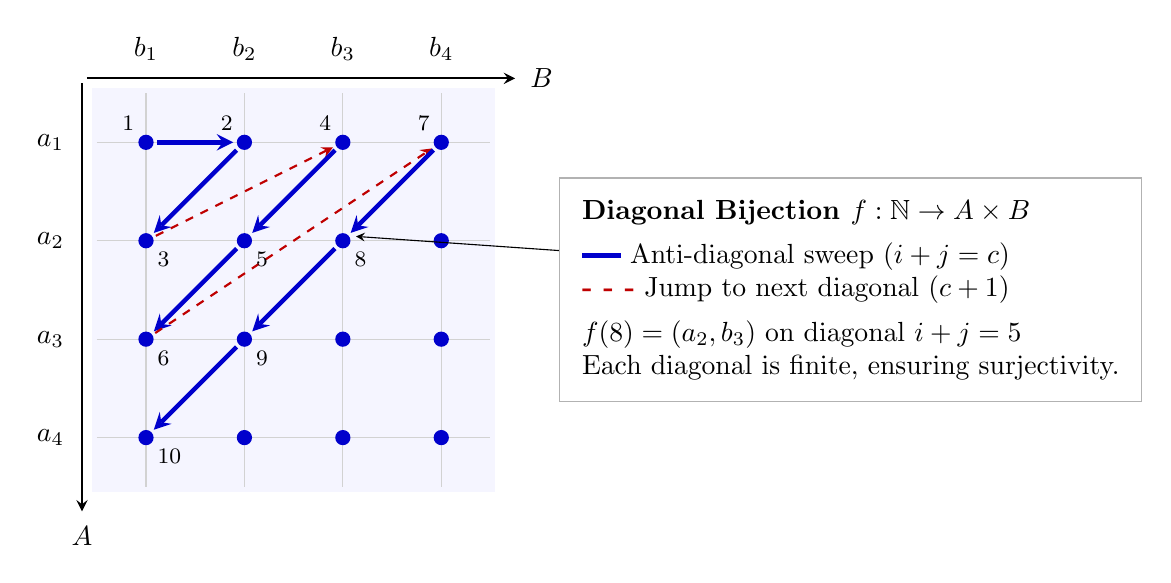
\begin{tikzpicture}[scale=1.25]
    % Layer 1: Background Fill
    \fill[blue!4] (0.45, 0.45) rectangle (4.55, 4.55);

    % Layer 2: Grid lines and Axes
    \draw[gray!35, thin] (0.5, 0.5) grid (4.5, 4.5);
    \draw[->, >=stealth, thick, black] (0.4, 4.65) -- (4.75, 4.65);
    \draw[->, >=stealth, thick, black] (0.35, 4.6) -- (0.35, 0.25);

    % Layer 3: Primary Diagonal Traversal Arrows (Down-left along i+j = c, and transitions)
    \draw[->, >=stealth, ultra thick, blue!80!black, shorten >=4pt, shorten <=4pt] (1, 4) -- (2, 4);
    \draw[->, >=stealth, ultra thick, blue!80!black, shorten >=4pt, shorten <=4pt] (2, 4) -- (1, 3);
    \draw[->, >=stealth, ultra thick, red!75!black, dashed, thick, shorten >=4pt, shorten <=4pt] (1, 3) -- (3, 4);
    \draw[->, >=stealth, ultra thick, blue!80!black, shorten >=4pt, shorten <=4pt] (3, 4) -- (2, 3);
    \draw[->, >=stealth, ultra thick, blue!80!black, shorten >=4pt, shorten <=4pt] (2, 3) -- (1, 2);
    \draw[->, >=stealth, ultra thick, red!75!black, dashed, thick, shorten >=4pt, shorten <=4pt] (1, 2) -- (4, 4);
    \draw[->, >=stealth, ultra thick, blue!80!black, shorten >=4pt, shorten <=4pt] (4, 4) -- (3, 3);
    \draw[->, >=stealth, ultra thick, blue!80!black, shorten >=4pt, shorten <=4pt] (3, 3) -- (2, 2);
    \draw[->, >=stealth, ultra thick, blue!80!black, shorten >=4pt, shorten <=4pt] (2, 2) -- (1, 1);

    % Lattice points
    \foreach \x in {1,2,3,4} {
        \foreach \y in {1,2,3,4} {
            \fill[blue!80!black] (\x, \y) circle (2.2pt);
        }
    }

    % Off-axis callout arrow
    \draw[->, >=stealth, thin, black, shorten >=3pt] (5.2, 2.9) -- (3.05, 3.05);

    % Layer 4: Nodes and Single-Node Multiline Legend
    \node[black, above=3pt] at (1, 4.65) {$b_1$};
    \node[black, above=3pt] at (2, 4.65) {$b_2$};
    \node[black, above=3pt] at (3, 4.65) {$b_3$};
    \node[black, above=3pt] at (4, 4.65) {$b_4$};
    \node[black, right=2pt] at (4.75, 4.65) {$B$};

    \node[black, left=3pt] at (0.35, 4) {$a_1$};
    \node[black, left=3pt] at (0.35, 3) {$a_2$};
    \node[black, left=3pt] at (0.35, 2) {$a_3$};
    \node[black, left=3pt] at (0.35, 1) {$a_4$};
    \node[black, below=2pt] at (0.35, 0.25) {$A$};

    \node[black, above left=1pt] at (1, 4) {\footnotesize $1$};
    \node[black, above left=1pt] at (2, 4) {\footnotesize $2$};
    \node[black, below right=1pt] at (1, 3) {\footnotesize $3$};
    \node[black, above left=1pt] at (3, 4) {\footnotesize $4$};
    \node[black, below right=1pt] at (2, 3) {\footnotesize $5$};
    \node[black, below right=1pt] at (1, 2) {\footnotesize $6$};
    \node[black, above left=1pt] at (4, 4) {\footnotesize $7$};
    \node[black, below right=1pt] at (3, 3) {\footnotesize $8$};
    \node[black, below right=1pt] at (2, 2) {\footnotesize $9$};
    \node[black, below right=1pt] at (1, 1) {\footnotesize $10$};

    \node[draw=gray!60, fill=white, align=left, inner sep=8pt, anchor=west, text=black] at (5.2, 2.5) {%
        \textbf{Diagonal Bijection $f: \mathbb{N} \to A \times B$}\\[4pt]
        $\textcolor{blue!80!black}{\rule[2pt]{14pt}{1.8pt}}$\ Anti-diagonal sweep ($i + j = c$)\\
        $\textcolor{red!75!black}{\textbf{- - -}}$\ Jump to next diagonal ($c + 1$)\\[4pt]
        $\displaystyle f(8) = (a_2, b_3)$ on diagonal $i + j = 5$\\
        Each diagonal is finite, ensuring surjectivity.%
    };
\end{tikzpicture}
\caption{Cantor's diagonal enumeration of $A \times B$ (Result 11.6). Because every anti-diagonal $i + j = c$ contains only $c - 1$ pairs, every element $(a_i, b_j)$ is reached at a finite index $n \in \mathbb{N}$.}
\label{fig:cantor_zigzag}
\end{figure}

\begin{figure}[htbp]
\centering
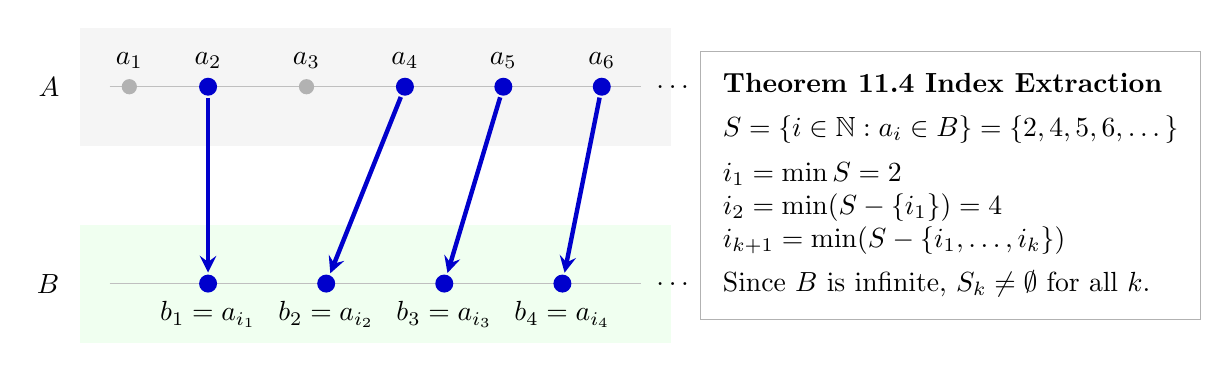
\begin{tikzpicture}[scale=1.25]
    % Layer 1: Background Fills
    \fill[gray!8] (-0.3, 2.4) rectangle (5.7, 3.6);
    \fill[green!6] (-0.3, 0.4) rectangle (5.7, 1.6);

    % Layer 2: Horizontal reference lines and tick marks
    \draw[gray!50, thin] (0, 3.0) -- (5.4, 3.0);
    \draw[gray!50, thin] (0, 1.0) -- (5.4, 1.0);

    % Layer 3: Extraction arrows from A (indices in S) to B
    \draw[->, >=stealth, ultra thick, blue!80!black, shorten >=4pt, shorten <=4pt] (1.0, 3.0) -- (1.0, 1.0);
    \draw[->, >=stealth, ultra thick, blue!80!black, shorten >=4pt, shorten <=4pt] (3.0, 3.0) -- (2.2, 1.0);
    \draw[->, >=stealth, ultra thick, blue!80!black, shorten >=4pt, shorten <=4pt] (4.0, 3.0) -- (3.4, 1.0);
    \draw[->, >=stealth, ultra thick, blue!80!black, shorten >=4pt, shorten <=4pt] (5.0, 3.0) -- (4.6, 1.0);

    % Dots in A (gray for non-B, blue for B)
    \fill[gray!60] (0.2, 3.0) circle (2.2pt);
    \fill[blue!80!black] (1.0, 3.0) circle (2.6pt);
    \fill[gray!60] (2.0, 3.0) circle (2.2pt);
    \fill[blue!80!black] (3.0, 3.0) circle (2.6pt);
    \fill[blue!80!black] (4.0, 3.0) circle (2.6pt);
    \fill[blue!80!black] (5.0, 3.0) circle (2.6pt);

    % Dots in B
    \fill[blue!80!black] (1.0, 1.0) circle (2.6pt);
    \fill[blue!80!black] (2.2, 1.0) circle (2.6pt);
    \fill[blue!80!black] (3.4, 1.0) circle (2.6pt);
    \fill[blue!80!black] (4.6, 1.0) circle (2.6pt);

    % Layer 4: Labels and Single-Node Multiline Legend
    \node[black, left=4pt] at (-0.3, 3.0) {$A$};
    \node[black, left=4pt] at (-0.3, 1.0) {$B$};

    \node[black, above=3pt] at (0.2, 3.0) {$a_1$};
    \node[black, above=3pt] at (1.0, 3.0) {$a_2$};
    \node[black, above=3pt] at (2.0, 3.0) {$a_3$};
    \node[black, above=3pt] at (3.0, 3.0) {$a_4$};
    \node[black, above=3pt] at (4.0, 3.0) {$a_5$};
    \node[black, above=3pt] at (5.0, 3.0) {$a_6$};
    \node[black, right=2pt] at (5.4, 3.0) {$\dots$};

    \node[black, below=3pt] at (1.0, 1.0) {$b_1 = a_{i_1}$};
    \node[black, below=3pt] at (2.2, 1.0) {$b_2 = a_{i_2}$};
    \node[black, below=3pt] at (3.4, 1.0) {$b_3 = a_{i_3}$};
    \node[black, below=3pt] at (4.6, 1.0) {$b_4 = a_{i_4}$};
    \node[black, right=2pt] at (5.4, 1.0) {$\dots$};

    \node[draw=gray!60, fill=white, align=left, inner sep=8pt, anchor=west, text=black] at (6.0, 2.0) {%
        \textbf{Theorem 11.4 Index Extraction}\\[4pt]
        $\displaystyle S = \{i \in \mathbb{N} : a_i \in B\} = \{2, 4, 5, 6, \dots\}$\\[4pt]
        $i_1 = \min S = 2$\\
        $i_2 = \min(S - \{i_1\}) = 4$\\
        $i_{k+1} = \min(S - \{i_1, \dots, i_k\})$\\[4pt]
        Since $B$ is infinite, $S_k \neq \emptyset$ for all $k$.%
    };
\end{tikzpicture}
\caption{Visualizing the Well-Ordering construction in Theorem 11.4. Compressing the sparse infinite subsequence $\{a_{i_k}\}$ closes all gaps without losing any element of $B$.}
\label{fig:well_ordering_extraction}
\end{figure}

\subsection{Heuristics and ``Cheats''}

\begin{itemize}
    \item \textbf{The ``Embed and Show Infinite'' Shortcut:} Almost any problem asking to prove a set $S$ is denumerable (where $S$ is defined by an inequality or restriction on integers/rationals, like Exercises 11.12, 11.14, 11.15, 11.17) does \textit{not} require constructing a closed-form bijection $\mathbb{N} \to S$. Simply find a denumerable superset (usually $\mathbb{N}$, $\mathbb{Z}$, $\mathbb{N} \times \mathbb{N}$, or $\mathbb{Q}$), prove $S$ is infinite by fixing one coordinate and letting the other vary over $\mathbb{N}$, and invoke Theorem 11.4.
    \item \textbf{Testing for Denumerability via Finite-Length Coordinates:} If every element of $S$ can be uniquely encoded by a fixed finite tuple of integers or rationals $(z_1, z_2, \dots, z_d) \in \mathbb{Z}^d$, then $S$ is countable. If $S$ is also infinite, $S$ is immediately denumerable.
    \item \textbf{Checking Bijections at Boundary Cases:} When grading or checking your own bijection $f : \mathbb{N} \to S$, always evaluate $f(1), f(2), f(3)$ and check whether $0$ or negative integers are accidentally included or omitted (e.g., in Exercise 11.8, verify $f(1) = 0$ and $f(2) = 1$).
\end{itemize}

\subsection{Pitfalls and Fallacies}

\begin{itemize}
    \item \textbf{The ``Infinite Row'' Trap:} Never enumerate a 2D array row-by-row or column-by-column. If row $1$ is infinite, an enumeration of row $1$ already uses all of $\mathbb{N}$, so row $2$ is never reached ($f$ fails surjectivity). Always sweep along \textit{finite} slices (anti-diagonals $i + j = c$ or boxes $\max(i, j) = c$).
    \item \textbf{Duplicate Representations Violating Injectivity:} In sets like $\mathbb{Q}^+$ (Result 11.7) or unordered subsets (Exercise 11.12), distinct pairs $(i, j)$ can represent the same mathematical object ($1/2 = 2/4$ or $\{1, 2\} = \{2, 1\}$). Failing to either skip duplicates or restrict to canonical representatives breaks injectivity.
    \item \textbf{Forgetting to Prove Infiniteness Before Invoking Theorem 11.4:} Theorem 11.4 states that every \textit{infinite} subset of a denumerable set is denumerable. A subset $B \subseteq A$ could be finite (even empty!), so proving $B$ is infinite is mandatory.
    \item \textbf{Confusing ``Denumerable'' with ``Countable'':} In Exercise 11.11, if $f : A \to B$ is injective and $B$ is denumerable, $A$ is \textit{countable}, not necessarily denumerable---$A$ could easily be finite (e.g., $|A| = 1$).
    \item \textbf{Assuming ``$A$ is infinite'' implies ``$A$ is denumerable'':} Every denumerable set is infinite, but the converse is false! Uncountable infinite sets (such as $\mathbb{R}$ or $\mathcal{P}(\mathbb{N})$) cannot be put in bijection with $\mathbb{N}$.
\end{itemize}

% ==============================================================================
% PART 5
% ==============================================================================
\section{Conceptual Synthesis and The ``Big Picture''}

\subsection{Thematic Connections}

The unifying theme of Section 11.2 is \textbf{structural invariance under countable indexing}: the remarkable stability of the lowest infinite cardinal $\aleph_0 = |\mathbb{N}|$ under set-theoretic operations. While finite cardinalities grow strictly under addition ($n + m > n$), multiplication ($n \cdot m > n$), and proper containment ($|B| < |A|$ for $B \subsetneq A$), the cardinal $\aleph_0$ absorbs finite shifts (Exercise 11.5), finite doubling (Exercise 11.10), countable unions (Exercise 11.16), and finite Cartesian products (Result 11.6, Exercise 11.18):
\[
\aleph_0 + 1 = \aleph_0, \qquad \aleph_0 + \aleph_0 = \aleph_0, \qquad \aleph_0 \cdot \aleph_0 = \aleph_0.
\]
Crucially, this theme exposes a profound distinction between \textit{order/topology} and \textit{cardinality}. The rational numbers $\mathbb{Q}$ are topologically dense in $\mathbb{R}$ (every open interval contains infinitely many rationals), whereas $\mathbb{N}$ is discrete and isolated. Yet set-theoretically, $|\mathbb{Q}| = |\mathbb{N}|$: density does not create uncountability.

\subsection{Forward and Backward Links}

\begin{itemize}
    \item \textbf{Backward Links (How Denumerable Sets Extend Prior Topics):}
    Denumerable sets synthesize three foundational pillars from earlier discrete mathematics: (1) \textit{functions} (injections, surjections, bijections, and compositions from Chapter 9), (2) \textit{equivalence relations} (numerical equivalence $|A| = |B|$ from Section 11.1 partitions the universe of sets into cardinality classes, with $[\mathbb{N}]$ being the class of denumerable sets), and (3) \textit{induction and the Well-Ordering Principle} on $\mathbb{N}$ (which provide the constructive engine for Theorem 11.4 and Exercise 11.18).
    
    \item \textbf{Forward Links (How Denumerable Sets Serve as a Bedrock for Advanced Theory):}
    \begin{enumerate}[label=(\roman*)]
        \item \textit{Uncountable Sets and Cantor's Diagonal Argument (Section 11.3):} Denumerable sets provide the exact baseline against which uncountability is defined. Proving $(0, 1)$ or $\mathbb{R}$ is uncountable proceeds by assuming it is denumerable ($[a_1, a_2, \dots]$) and constructing a contradiction.
        \item \textit{Measure Theory and Lebesgue Integration:} The fundamental axiom of probability and measure theory is \textbf{countable additivity} ($\sigma$-additivity): $\mu\left(\bigcup_{i=1}^\infty E_i\right) = \sum_{i=1}^\infty \mu(E_i)$ for pairwise disjoint measurable sets (precisely the structure of Exercise 11.16). Because $\mathbb{Q}$ is denumerable, $\mathbb{Q}$ can be covered by a countable union of open intervals of total length $\varepsilon > 0$, proving $\mathbb{Q}$ has Lebesgue measure zero despite being dense in $\mathbb{R}$!
        \item \textit{Separable Hilbert Spaces and Functional Analysis:} A Banach or Hilbert space (such as $L^2([0,1])$) is \textbf{separable} if it contains a countable dense subset (e.g., polynomials with rational coefficients, whose denumerability follows from $\mathbb{Q}$ and finite products). Separability guarantees the existence of a countable orthonormal basis $\{e_n\}_{n \in \mathbb{N}}$, enabling Fourier analysis and spectral decompositions in PDEs and stochastic calculus.
        \item \textit{Computability Theory:} The set of all finite strings over a finite alphabet (and hence all Turing machines, Python programs, and formal mathematical proofs) is denumerable. Since the set of all functions $\mathbb{N} \to \{0, 1\}$ is uncountable, almost all mathematical functions are non-computable!
    \end{enumerate}
\end{itemize}

% ==============================================================================
% PART 6
% ==============================================================================
\section{Abstract Real-World Modeling (AI, ML, and Quant Finance)}

\subsection{Concrete Scenarios}

\begin{enumerate}[label=\textbf{\arabic*.}]
    \item \textbf{Statistical Learning Theory and Occam's Razor over Countable Hypothesis Spaces (AI/ML):}
    In Machine Learning, Empirical Risk Minimization (ERM) seeks a predictor $h \in \mathcal{H}$ minimizing training error. If $\mathcal{H}$ is uncountable with infinite VC-dimension, uniform convergence fails without strong geometric constraints. However, every implementable model class on a digital computer---such as all neural networks of arbitrary finite depth and width with rational weights $w \in \mathbb{Q}$, or all finite-length programs/decision trees---is a countable union of finite-dimensional rational spaces $\mathcal{H} = \bigcup_{d=1}^\infty \mathcal{H}_d$, and is therefore \textbf{denumerable} (by Result 11.8 and Exercise 11.16/Section 7.1). Because $\mathcal{H}$ is denumerable, we can assign a strictly positive prior weight $p(h) > 0$ to every $h \in \mathcal{H}$ with $\sum_{h \in \mathcal{H}} p(h) = 1$, enabling the **countable union bound** for non-uniform PAC generalization guarantees and Structural Risk Minimization (SRM).

    \item \textbf{Limit Order Book (LOB) Dynamics as a Denumerable-State Markov Decision Process (Quant Finance):}
    In modern algorithmic trading and optimal execution, asset prices do not move continuously on $\mathbb{R}$; exchanges enforce a discrete tick size $\Delta p > 0$, confining mid-prices to a discrete lattice $\mathcal{P} = \{k \Delta p : k \in \mathbb{N}\}$, while order queue volumes at the best $d$ bid/ask levels lie in $\mathbb{Z}_{\geq 0}^d$. Even though price levels and queue depths are theoretically unbounded above, the state space $\mathcal{S} = \mathbb{N} \times \mathbb{Z}_{\geq 0}^{2d}$ is a finite Cartesian product of denumerable sets, hence **denumerable** (extending Result 11.6). This guarantees that the discrete-time transition kernel $P(s' \mid s, a)$ is an infinite stochastic matrix rather than a Radon-Nikodym density, avoiding non-measurable set pathologies (since the discrete $\sigma$-algebra $\mathcal{F} = \mathcal{P}(\mathcal{S})$ makes every subset measurable) and reducing Bellman expectation operators to convergent infinite series.

    \item \textbf{Countable-State Continuous-Time Markov Chains in Credit and Queueing Risk (Quant Finance):}
    In modeling multi-order-book queueing imbalances or birth-death credit default intensities over an infinite state ladder $\mathcal{S} = \mathbb{Z}_{\geq 0}$, Kolmogorov's forward equations $\frac{d}{dt} P_{ij}(t) = \sum_{k \in \mathcal{S}} P_{ik}(t) Q_{kj}$ rely critically on enumerating $\mathcal{S}$ via a bijection $\phi : \mathbb{N} \to \mathcal{S}$ and interchanging differentiation with countable summation over $\mathbb{N}$.
\end{enumerate}

\subsection{Model Problem Setup: Structural Risk Minimization over a Denumerable Hypothesis Space}

We now formalize Scenario 1 as a rigorous quantitative statistical learning framework, explicitly grounded in probability spaces and denumerable set theory.

\subsubsection*{1. Data Probability Space}
Let $\mathcal{X} \subseteq \mathbb{R}^p$ be an input feature space and $\mathcal{Y} = \{0, 1\}$ (or bounded $[0, 1]$) be the label space. Let $(\Omega, \mathcal{F}, \mathbb{P})$ be a complete probability space supporting an i.i.d.\ sample $S_m = ((X_1, Y_1), \dots, (X_m, Y_m)) \sim \mathcal{D}^m$, where $\mathcal{D}$ is an unknown probability distribution on $(\mathcal{X} \times \mathcal{Y}, \mathcal{B}(\mathcal{X}) \otimes \mathcal{P}(\mathcal{Y}))$.

\subsubsection*{2. Construction of the Denumerable Hypothesis Space $\mathcal{H}$}
Consider the hierarchy of finite-width rational-parameterized predictors: for each complexity tier $d \in \mathbb{N}$, let
\[
\mathcal{H}_d = \left\{ h_\theta : \mathcal{X} \to [0, 1] \;\middle|\; \theta \in \mathbb{Q}^d \right\}
\]
be the family of predictors (e.g., quantized neural networks or rational linear/polynomial classifiers) indexed by $d$ rational parameters.
\begin{itemize}
    \item Since $\mathbb{Q}$ is denumerable (Result 11.8), an immediate induction on $d$ using Result 11.6 shows that $\mathbb{Q}^d$ is denumerable for every $d \in \mathbb{N}$. Assuming distinct parameters or canonicalizing duplicates yields $|\mathcal{H}_d| \leq |\mathbb{N}|$.
    \item Define the universal implementable hypothesis space as $\mathcal{H} = \bigcup_{d=1}^\infty \mathcal{H}_d$. Since $\mathcal{H}$ is a countable union of countable sets (extending Exercise 11.16), there exists an explicit bijection $\phi : \mathbb{N} \to \mathcal{H}$ indexing every hypothesis as $h_k = \phi(k)$ for $k \in \mathbb{N}$.
\end{itemize}

\subsubsection*{3. Countable Prior and Kolmogorov Complexity Weighting}
Because $\mathcal{H}$ is denumerable, we can define a valid probability mass function (prior) $P : \mathcal{H} \to (0, 1)$ over the discrete $\sigma$-algebra $\mathcal{P}(\mathcal{H})$ via the bijection $\phi^{-1}$ (or prefix-free description length $L(h) \in \mathbb{N}$ satisfying Kraft's inequality):
\[
P(h_k) = \frac{6}{\pi^2 k^2} \quad (\text{so } \sum_{k=1}^\infty P(h_k) = 1), \qquad \text{or} \qquad P(h) = 2^{-L(h)} \text{ with } \sum_{h \in \mathcal{H}} 2^{-L(h)} \leq 1.
\]
(Note that no strictly positive probability measure $P(h) > 0$ for all $h \in \mathcal{H}$ could sum to $1$ if $\mathcal{H}$ were uncountable!)

\subsubsection*{4. Loss Function, Generalization Bound, and Optimization Problem}
For a bounded loss $\ell : [0, 1] \times [0, 1] \to [0, 1]$, define the true population risk and empirical risk of $h \in \mathcal{H}$:
\[
R(h) = \mathbb{E}_{(X, Y) \sim \mathcal{D}}[\ell(h(X), Y)], \qquad \widehat{R}_m(h) = \frac{1}{m} \sum_{i=1}^m \ell(h(X_i), Y_i).
\]
For each $h_k \in \mathcal{H}$ ($k \in \mathbb{N}$) and confidence $\delta \in (0, 1)$, set $\delta_k = \delta \cdot P(h_k)$ and define the failure event
\[
E_k = \left\{ \omega \in \Omega : R(h_k) - \widehat{R}_m(h_k)(\omega) > \sqrt{\frac{\ln(1/P(h_k)) + \ln(1/\delta)}{2m}} \right\}.
\]
By Hoeffding's inequality, $\mathbb{P}(E_k) \leq \delta_k = \delta P(h_k)$. Invoking \textbf{countable subadditivity} of the probability measure $\mathbb{P}$ over the denumerable index set $\mathbb{N}$:
\[
\mathbb{P}\left(\bigcup_{k=1}^\infty E_k\right) \leq \sum_{k=1}^\infty \mathbb{P}(E_k) \leq \sum_{k=1}^\infty \delta P(h_k) = \delta \sum_{k=1}^\infty P(h_k) \leq \delta.
\]
Taking the complement, with probability at least $1 - \delta$ over $S_m \sim \mathcal{D}^m$, \textit{simultaneously for all} $h \in \mathcal{H}$:
\[
R(h) \leq \widehat{R}_m(h) + \sqrt{\frac{\ln(1/P(h)) + \ln(1/\delta)}{2m}}.
\]
This directly yields the \textbf{Structural Risk Minimization (SRM) Optimization Problem}:
\[
\hat{h}_{\mathrm{SRM}} \in \arg\min_{h \in \mathcal{H}} \left\{ \frac{1}{m} \sum_{i=1}^m \ell(h(X_i), Y_i) + \sqrt{\frac{\ln(1/P(h)) + \ln(1/\delta)}{2m}} \right\},
\]
where the penalty $\ln(1/P(h)) = L(h)\ln 2$ (or $2\ln \phi^{-1}(h) + \ln(\pi^2/6)$) exists and yields a non-vacuous bound \textit{precisely} because $\mathcal{H}$ is denumerable.

% ==============================================================================
% PART 7
% ==============================================================================
\section{Common Variations and Untested Concepts}

Several fundamental theorems on denumerable and countable sets do not appear directly in the Section 11.2 exercises, yet are essential in university-level analysis and discrete mathematics.

\subsection{General Countable Unions of Countable Sets (Non-Disjoint Case)}

Exercise 11.16 required the sets $A_1, A_2, \dots$ to be \textit{pairwise disjoint} and \textit{denumerable}. In practice, collections overlap and may include finite or empty sets.

\begin{theorem}[General Countable Union]
Let $I$ be a nonempty countable index set, and for each $i \in I$, let $A_i$ be a countable set. Then $U = \bigcup_{i \in I} A_i$ is countable.
\end{theorem}

\begin{proof}[Proof (Canonical Index Injection into $\mathbb{N} \times \mathbb{N}$)]
If $U = \emptyset$, then $U$ is finite and hence countable. Assume $U \neq \emptyset$. Since $I$ is countable and nonempty, there exists an injection $\alpha : I \to \mathbb{N}$ (either $I = \{i_1, \dots, i_k\}$ or $I$ is denumerable). Likewise, for each $i \in I$, since $A_i$ is countable, there exists an injection $\beta_i : A_i \to \mathbb{N}$ (using Countable Choice).

For each element $x \in U$, the set $I_x = \{i \in I : x \in A_i\}$ is nonempty, so $\{\alpha(i) : i \in I_x\}$ is a nonempty subset of $\mathbb{N}$. By the Well-Ordering Principle, there is a unique index $i_x \in I_x$ minimizing $\alpha(i_x)$. Define $F : U \to \mathbb{N} \times \mathbb{N}$ by
\[
F(x) = \bigl(\alpha(i_x),\, \beta_{i_x}(x)\bigr).
\]
We claim $F$ is injective: if $F(x) = F(y)$, then $\alpha(i_x) = \alpha(i_y)$ and $\beta_{i_x}(x) = \beta_{i_y}(y)$. Since $\alpha$ is injective, $i_x = i_y$; calling this common index $i^*$, we have $\beta_{i^*}(x) = \beta_{i^*}(y)$. Since $\beta_{i^*}$ is injective, $x = y$.

Thus $F$ is a bijection from $U$ onto $F(U) \subseteq \mathbb{N} \times \mathbb{N}$. Since $\mathbb{N} \times \mathbb{N}$ is denumerable (Result 11.6), $F(U)$ is either finite or (by Theorem 11.4) denumerable, so $U$ is countable. $\blacksquare$
\end{proof}

\subsection{The Set of All Finite Subsets of $\mathbb{N}$}

Exercise 11.12 proved that $2$-element subsets of $\mathbb{N}$ are denumerable. Remarkably, the set of \textit{all} finite subsets of $\mathbb{N}$ is also denumerable (whereas the full power set $\mathcal{P}(\mathbb{N})$ is uncountable).

\begin{theorem}[Denumerability of $\mathcal{P}_{\mathrm{fin}}(\mathbb{N})$]
Let $\mathcal{P}_{\mathrm{fin}}(\mathbb{N}) = \{S \subseteq \mathbb{N} : S \text{ is finite}\}$. Then $\mathcal{P}_{\mathrm{fin}}(\mathbb{N})$ is denumerable.
\end{theorem}

\begin{proof}[Proof (Binary Representation Bijection)]
Define $f : \mathcal{P}_{\mathrm{fin}}(\mathbb{N}) \to \mathbb{N}$ by
\[
f(S) = 1 + \sum_{k \in S} 2^{k - 1},
\]
with the convention that the empty sum is $0$, so $f(\emptyset) = 1$. Since $S$ is finite, the sum has finitely many terms and $f(S) \in \mathbb{N}$. By the uniqueness of binary (base-$2$) representations of non-negative integers:
\begin{itemize}
    \item \textit{Injectivity:} If $f(S_1) = f(S_2)$, then $\sum_{k \in S_1} 2^{k-1} = \sum_{k \in S_2} 2^{k-1}$. Because every non-negative integer has a unique binary expansion (where the $(k-1)$-th bit is $1$ if and only if $k \in S$), we must have $S_1 = S_2$.
    \item \textit{Surjectivity:} For any $m \in \mathbb{N}$, the integer $m - 1 \geq 0$ has a finite binary representation $m - 1 = \sum_{j=0}^{r} c_j 2^j$ with $c_j \in \{0, 1\}$. Setting $S = \{j + 1 : c_j = 1\} \in \mathcal{P}_{\mathrm{fin}}(\mathbb{N})$, we obtain $f(S) = 1 + (m - 1) = m$.
\end{itemize}
Thus $f$ is a bijection, proving $\mathcal{P}_{\mathrm{fin}}(\mathbb{N})$ is denumerable. $\blacksquare$
\end{proof}

\subsection{Denumerability of Polynomials $\mathbb{Z}[x]$ and Algebraic Numbers $\overline{\mathbb{Q}}$}

\begin{theorem}[Algebraic Numbers are Denumerable]
Let $\overline{\mathbb{Q}}$ be the set of all complex (or real) algebraic numbers---numbers that are roots of some nonzero polynomial with integer coefficients. Then $\overline{\mathbb{Q}}$ is denumerable.
\end{theorem}

\begin{proof}[Proof (Height / Degree Stratification)]
For each $d \in \mathbb{Z}_{\geq 0}$, let $P_d = \{a_d x^d + \dots + a_1 x + a_0 : a_i \in \mathbb{Z},\ a_d \neq 0\}$ be the set of integer polynomials of exact degree $d$. There is an obvious bijection between $P_d$ and $(\mathbb{Z} - \{0\}) \times \mathbb{Z}^d$, which is denumerable by Result 11.3, Theorem 11.4, and induction on Result 11.6. Hence each $P_d$ ($d \geq 1$) is denumerable, and the set of all nonzero polynomials $P = \bigcup_{d=1}^\infty P_d$ is denumerable by Exercise 11.16 (as $P_d$ are pairwise disjoint by degree).

For each $p \in P$, let $R(p) = \{z \in \mathbb{C} : p(z) = 0\}$ be its set of roots. By the Fundamental Theorem of Algebra (or factor theorem), if $\deg(p) = d$, then $|R(p)| \leq d$, so $R(p)$ is finite. Now $\overline{\mathbb{Q}} = \bigcup_{p \in P} R(p)$ is a countable union of finite sets, hence countable by Theorem 7.1. Finally, since $\mathbb{Q} \subseteq \overline{\mathbb{Q}}$ (each $q \in \mathbb{Q}$ is a root of $x - q$ or $bx - a$) and $\mathbb{Q}$ is infinite, $\overline{\mathbb{Q}}$ is infinite, and therefore denumerable. $\blacksquare$
\end{proof}

\subsection{Every Infinite Set Contains a Denumerable Subset}

\begin{theorem}[Denumerable Subset Extraction]
Every infinite set $X$ contains a denumerable subset. Consequently, for any infinite set $X$ and any element $y \notin X$, $|X| = |X \cup \{y\}|$.
\end{theorem}

\begin{proof}[Proof (Recursive Extraction and Hilbert Shift)]
Since $X$ is infinite, $X \neq \emptyset$, so we may choose $x_1 \in X$. Inductively, once distinct elements $x_1, \dots, x_k \in X$ have been chosen, the set $X - \{x_1, \dots, x_k\}$ must be nonempty (otherwise $X = \{x_1, \dots, x_k\}$ would be finite). Using Countable Choice, pick $x_{k+1} \in X - \{x_1, \dots, x_k\}$. Thus $D = \{x_1, x_2, x_3, \dots\} \subseteq X$ is a denumerable subset of $X$.

Now let $y \notin X$. Define $f : X \cup \{y\} \to X$ by $f(y) = x_1$, $f(x_n) = x_{n+1}$ for all $n \in \mathbb{N}$, and $f(z) = z$ for all $z \in X - D$. Because $X = (X - D) \sqcup D$ and $f$ maps $X - D$ identically to $X - D$ while mapping $\{y\} \cup D$ bijectively onto $D$, $f$ is a bijection, proving $|X \cup \{y\}| = |X|$. $\blacksquare$
\end{proof}

% ==============================================================================
% PART 8
% ==============================================================================
\section{Advanced Diagnostic Testing: ``Find the Flaw''}

Each of the following five proofs appears rigorous at first glance, yet contains a single, subtle, fatal mathematical or logical flaw. Identify the exact error, explain why it invalidates the proof, and provide the corrected step. Check your work against the Solution Key at the end of this section.

\subsection{Diagnostic Problem 1: Row-by-Row Enumeration of $\mathbb{N} \times \mathbb{N}$}
\textbf{Claim:} $\mathbb{N} \times \mathbb{N}$ is denumerable.\\
\textbf{Proposed Proof:} Arrange $\mathbb{N} \times \mathbb{N}$ in an infinite grid where row $i$ contains $(i, 1), (i, 2), (i, 3), \dots$ for each $i \in \mathbb{N}$. We construct a bijection $f : \mathbb{N} \to \mathbb{N} \times \mathbb{N}$ sequentially: first map $1, 2, 3, \dots$ onto the entire first row $(1, 1), (1, 2), (1, 3), \dots$; once the first row is completely listed, continue mapping the subsequent natural numbers onto row $2$, namely $(2, 1), (2, 2), \dots$, then row $3$, and so on. Because every row is visited in order and no ordered pair is listed twice, $f$ is both one-to-one and onto. Therefore $\mathbb{N} \times \mathbb{N}$ is denumerable. $\blacksquare$

\subsection{Diagnostic Problem 2: Direct Grid Bijection for $\mathbb{Q}^+$}
\textbf{Claim:} The set $\mathbb{Q}^+$ of positive rational numbers is denumerable.\\
\textbf{Proposed Proof:} Consider the infinite array where row $i$ and column $j$ ($i, j \in \mathbb{N}$) contains the rational number $j/i$. Traverse the array along finite anti-diagonals $i + j = c$ for $c = 2, 3, 4, \dots$, defining a function $f : \mathbb{N} \to \mathbb{Q}^+$ by recording each entry in order of traversal:
\[
f(1) = \frac{1}{1},\quad f(2) = \frac{2}{1},\quad f(3) = \frac{1}{2},\quad f(4) = \frac{3}{1},\quad f(5) = \frac{2}{2},\quad f(6) = \frac{1}{3},\quad \dots
\]
Since every positive rational number $p/q$ lies in row $q$, column $p$, and each anti-diagonal $i + j = c$ has finitely many entries ($c - 1$), every element of $\mathbb{Q}^+$ is reached at some finite index $n \in \mathbb{N}$, so $f$ is onto. Moreover, each position $(i, j)$ in the grid is visited at most once, so $f$ is one-to-one. Hence $f$ is bijective and $\mathbb{Q}^+$ is denumerable. $\blacksquare$

\subsection{Diagnostic Problem 3: Arbitrary Nonempty Subsets of Denumerable Sets}
\textbf{Claim:} Every nonempty subset $B$ of a denumerable set $A$ is denumerable.\\
\textbf{Proposed Proof:} Let $A = \{a_1, a_2, a_3, \dots\}$ be denumerable and $B \subseteq A$ be nonempty. Define the index set $S = \{i \in \mathbb{N} : a_i \in B\}$. Since $B \neq \emptyset$, $S$ is a nonempty subset of $\mathbb{N}$. By the Well-Ordering Principle, $S$ has a smallest element $i_1$; set $b_1 = a_{i_1}$. Inductively, for each $k \geq 1$, having defined $i_1 < i_2 < \dots < i_k$ in $S$, let $S_k = S - \{i_1, \dots, i_k\}$ and define $i_{k+1} = \min S_k$ and $b_{k+1} = a_{i_{k+1}}$. Since $i_1 < i_2 < i_3 < \dots$ are strictly increasing, the elements $b_1, b_2, b_3, \dots$ are pairwise distinct. Finally, for any $b \in B$, $b = a_n$ for some $n \in S$, and since there are at most $n - 1$ elements of $S$ strictly less than $n$, $n = i_m$ for some $m \leq n$, so $b = b_m$. Thus $B = \{b_1, b_2, b_3, \dots\}$ is denumerable. $\blacksquare$

\subsection{Diagnostic Problem 4: Countability of the Power Set $\mathcal{P}(\mathbb{N})$}
\textbf{Claim:} The power set $\mathcal{P}(\mathbb{N})$ of all subsets of $\mathbb{N}$ is denumerable.\\
\textbf{Proposed Proof:} For each $k \in \mathbb{Z}_{\geq 0}$, let $\mathcal{P}_k(\mathbb{N})$ denote the set of all $k$-element subsets of $\mathbb{N}$. For $k = 0$, $\mathcal{P}_0(\mathbb{N}) = \{\emptyset\}$ is finite. For $k \geq 1$, every $k$-element subset $\{n_1, \dots, n_k\}$ with $n_1 < \dots < n_k$ corresponds bijectively to an increasing $k$-tuple in $\mathbb{N}^k$; by induction on Result 11.6 and Theorem 11.4, each $\mathcal{P}_k(\mathbb{N})$ ($k \geq 1$) is denumerable. Notice that the families $\{\mathcal{P}_k(\mathbb{N})\}_{k=0}^\infty$ are pairwise disjoint, and every subset of $\mathbb{N}$ has some size $k$, so
\[
\mathcal{P}(\mathbb{N}) = \bigcup_{k=0}^\infty \mathcal{P}_k(\mathbb{N}).
\]
Since a countable union of countable sets is countable (and $\mathcal{P}_1(\mathbb{N})$ is infinite), $\mathcal{P}(\mathbb{N})$ is denumerable. $\blacksquare$

\subsection{Diagnostic Problem 5: Inductive Enumeration of Any Infinite Set}
\textbf{Claim:} Every infinite set $B$ is denumerable.\\
\textbf{Proposed Proof:} Let $B$ be an arbitrary infinite set. Since $B$ is infinite, $B \neq \emptyset$, so we can pick an element $b_1 \in B$. Next, since $B$ is infinite, $B - \{b_1\}$ is nonempty, so we can pick $b_2 \in B - \{b_1\}$. Proceeding inductively, given distinct elements $b_1, b_2, \dots, b_k \in B$, the set $B - \{b_1, \dots, b_k\}$ cannot be empty (otherwise $B$ would have finite cardinality $k$), so we may choose $b_{k+1} \in B - \{b_1, \dots, b_k\}$. This defines an injective function $f : \mathbb{N} \to B$ via $f(n) = b_n$. Because $B$ is infinite and this process continues forever without ever terminating, every element of $B$ is eventually selected, giving $B = \{b_1, b_2, b_3, \dots\}$. Hence $B$ is denumerable. $\blacksquare$

\subsection{Solution Key}

\begin{enumerate}[label=\textbf{Flaw \arabic*:}]
    \item \textbf{Failure of Surjectivity After an Infinite First Row (Diagnostic Problem 1):}
    \begin{itemize}
        \item \textit{The Error:} The phrase ``once the first row is completely listed, continue onto row $2$'' is logically impossible for a map $f : \mathbb{N} \to \mathbb{N} \times \mathbb{N}$. The first row $\{(1, j) : j \in \mathbb{N}\}$ already requires every $n \in \mathbb{N}$ ($f(n) = (1, n)$), leaving no natural numbers remaining to map to row $2$.
        \item \textit{Why It Fails:} Surjectivity fails completely: no $n \in \mathbb{N}$ satisfies $f(n) = (2, 1)$. (Mathematically, this describes an ordinal indexing of type $\omega + \omega + \dots = \omega^2$, not $\omega = \mathbb{N}$.)
        \item \textit{Correction:} Traverse the grid along \textit{finite} anti-diagonals $i + j = c$ (Result 11.6) or use the closed-form bijection $f^{-1}(m, n) = 2^{m-1}(2n - 1)$ (Exercise 11.18).
    \end{itemize}

    \item \textbf{Failure of Injectivity Due to Unreduced Fractions (Diagnostic Problem 2):}
    \begin{itemize}
        \item \textit{The Error:} Visiting each grid coordinate $(i, j)$ at most once proves that the map $(i, j) \mapsto n$ is injective on \textit{coordinates} $\mathbb{N} \times \mathbb{N}$, not on \textit{values} in $\mathbb{Q}^+$.
        \item \textit{Why It Fails:} As elements of $\mathbb{Q}^+$, $f(1) = \frac{1}{1} = 1$ and $f(5) = \frac{2}{2} = 1$, so $f(1) = f(5)$ with $1 \neq 5$. Thus $f$ is not one-to-one.
        \item \textit{Correction:} Either skip any fraction $j/i$ equal to a previously listed value (as in Result 11.7), or restrict the grid so row $i$ contains only fractions $j/i$ with $\gcd(i, j) = 1$ (reduced to lowest terms).
    \end{itemize}

    \item \textbf{Omission of the Infiniteness Hypothesis for $S_k \neq \emptyset$ (Diagnostic Problem 3):}
    \begin{itemize}
        \item \textit{The Error:} In the inductive step, $i_{k+1} = \min S_k$ is asserted without verifying that $S_k = S - \{i_1, \dots, i_k\}$ is nonempty!
        \item \textit{Why It Fails:} The Well-Ordering Principle applies only to \textit{nonempty} subsets of $\mathbb{N}$. If $B$ is finite (e.g., $B = \{a_1, a_2\}$), then $S_2 = S - \{1, 2\} = \emptyset$, and $\min S_2$ does not exist. The claim itself is false for finite nonempty subsets $B \subseteq A$.
        \item \textit{Correction:} Restrict the claim to \textit{infinite} subsets $B \subseteq A$ (Theorem 11.4). Then $S$ is infinite, so removing finitely many elements $\{i_1, \dots, i_k\}$ leaves $S_k$ infinite (and hence nonempty), validly permitting $\min S_k$.
    \end{itemize}

    \item \textbf{Confusing $\mathcal{P}_{\mathrm{fin}}(\mathbb{N})$ with $\mathcal{P}(\mathbb{N})$ (Diagnostic Problem 4):}
    \begin{itemize}
        \item \textit{The Error:} The equality $\mathcal{P}(\mathbb{N}) = \bigcup_{k=0}^\infty \mathcal{P}_k(\mathbb{N})$ is false.
        \item \textit{Why It Fails:} While every finite subset of $\mathbb{N}$ has some cardinality $k \in \mathbb{Z}_{\geq 0}$, $\mathbb{N}$ also possesses \textit{infinite} subsets (such as $2\mathbb{N}$, the primes, or $\mathbb{N}$ itself). Thus $\bigcup_{k=0}^\infty \mathcal{P}_k(\mathbb{N}) = \mathcal{P}_{\mathrm{fin}}(\mathbb{N}) \subsetneq \mathcal{P}(\mathbb{N})$. Indeed, Cantor's Theorem proves $\mathcal{P}(\mathbb{N})$ is uncountable.
        \item \textit{Correction:} Replace $\mathcal{P}(\mathbb{N})$ in the claim with $\mathcal{P}_{\mathrm{fin}}(\mathbb{N})$, the set of all \textit{finite} subsets of $\mathbb{N}$, for which the proof is completely valid.
    \end{itemize}

    \item \textbf{Fallacy of ``Continuing Forever'' Implying Surjectivity (Diagnostic Problem 5):}
    \begin{itemize}
        \item \textit{The Error:} Concluding that ``because the selection process continues forever, every element of $B$ is eventually selected, so $B = \{b_1, b_2, \dots\}$.''
        \item \textit{Why It Fails:} Extracting $b_1, b_2, \dots$ only constructs an injection $f : \mathbb{N} \to B$, proving that $B$ contains a denumerable \textit{subset} $B' = \{b_1, b_2, \dots\} \subseteq B$. It does not prove $B \subseteq B'$ (surjectivity). Counterexample: if $B = \mathbb{R}$, one can pick $b_n = n$ forever, yet $\frac{1}{2} \in \mathbb{R}$ is never chosen.
        \item \textit{Correction:} Change the claim to ``Every infinite set $B$ contains a denumerable subset,'' and conclude only that $B' = \{b_1, b_2, b_3, \dots\} \subseteq B$ is denumerable (as in Theorem 7.4).
    \end{itemize}
\end{enumerate}

\end{document}